\section{Input/Output Methods}

References: Desoev, Vidyasagar "Feedback Systes Input-output properties"

\begin{tikzpicture}[auto,>=latex']
    \tikzstyle{block} = [draw, shape=rectangle, minimum height=3em, minimum width=3em, node distance=2cm, line width=1pt]
    \tikzstyle{sum} = [draw, shape=circle, node distance=1.5cm, line width=1pt, minimum width=1.25em]
    \tikzstyle{branch}=[fill,shape=circle,minimum size=4pt,inner sep=0pt]
    \tikzstyle{tmp} = [coordinate]
    %Creating Blocks and Connection Nodes
    \node at (-1.5,0) (input) {};
    \node [block] (sys) {System};
    \node at (1.5,0) (output) {};
    %Conecting Blocks
    \begin{scope}[line width=1pt]
         \draw[->] (input) -- node{$u$} (sys);
         \draw[->] (sys) -- node{$y$} (output);
    \end{scope}
\end{tikzpicture}

\begin{equation*}
\begin{split}
&u: u\rightarrow y \\
&u,y:[0,\infty]\rightarrow \mathbb{R}^m \\
&t \rightarrow u(t), y(t)
\end{split}
\end{equation*}

\subsection{Sygnals and Systems}

\begin{itemize}
\item How to define "stability" in input/output setting?
\item Which signals are "good"?
\end{itemize}

\begin{Definition}
 $Lp$-spaces, $p\in[1,\infty]$. 
 $Lp[0,\infty) = \{\Phi:[0,\infty)\rightarrow\mathbb{R}^m, measurable|
  \int_0^\infty ||\Phi(t)||^p dt < \infty\}$
\end{Definition}

Interpretation: "finite energy signal" (p=2).

Remark: "measurable" = pointwise limit of a sequence of piecewise constant functions
(except on a set of measure 0)

\begin{Example}:

\begin{itemize}
 \item[-] continuous function
 \item[-] functions with "few enough" discontinuities
\end{itemize}
\end{Example}

$Lp$ is a real vector space ("signals $\Phi(\cdot)$ are vectors") i.e., for 
$\Phi, \Phi_1, \Phi_2 \in Lp$, $\alpha \in \mathbb{R}$ vector addition:
$\Phi_1+\Phi_2:t \rightarrow \Phi_1(t)+\Phi_2(t) \in Lp$. Scalar multiplication:
$\alpha \Phi:t\rightarrow \alpha\Phi(t) \in Lp$

Zero element is signal $\Phi \equiv 0$.

$Lp$ is a normed vector space with norm $||\Phi||_{Lp}=\sqrt[p]{\int_0^\infty ||\Phi(t)||^p dt}$
for $\Phi \in Lp$ $\Rightarrow$
\begin{itemize}
 \item $||\Phi||_{Lp}=0 \iff \Phi=0$, else $||\Phi||_{Lp}>0$
 \item for $\alpha \in \mathbb{R}$, $||\alpha\Phi||_{Lp}=|\alpha| ||\Phi||_{Lp}$
 \item for $\Phi_1, \Phi_2 \in Lp\ $ $||\Phi_1+\Phi_2||_{Lp} \le ||\Phi_1||_{Lp}+||\Phi_2||_{Lp}$
\end{itemize}

For $p \to \infty$ set of all measurable and (essentially) bounded functions $L_{\infty}$, for continuous $\phi$ 
\begin{equation*}
\|\phi\|_{L_{\infty}} = \inf \{ c \in \mathbb{R} | \|\phi(t)\| \leq c\ a.e.\} = \sup_{t > 0} \| \phi(t)\|
\end{equation*}

\begin{Example}
\begin{equation*}
\phi (t) = e^{- \alpha t}, \ \alpha > 0, \ p \in [1,\infty )
\end{equation*}
\begin{equation*}
\begin{split}
\|\phi \|_{L_p} = \sqrt[p]{\int_0^{\infty} \|e^{-\alpha t}\|^p dt} = \\
= \sqrt[p]{[-\frac{1}{\alpha p}e^{-\alpha pt}]_0^{\infty}} = \sqrt[p]{\frac{1}{\alpha p}} < \infty \\
\Rightarrow \phi \in L_p \ \forall p \in [1, \infty) \ p= \infty : \\
\sup_{t \geq 0} \phi (t) = \phi (0) = 1 \Rightarrow p \in L_{\infty}
\end{split}
\end{equation*}
\end{Example}

Special case $p = 2$ 

$L_2$ can be equipped with an inner product $\phi_1, \phi_2 \in L_2$, we write $<\phi_1, \phi_2>_{L_2} :=  \int_0^{\infty} \phi_1(t)^T\phi_2(t)dt$

symmetry $<\phi_1, \phi_2>_{L_2} = <\phi_2, \phi_1>_{L_2}$

(bi- )linearity 
\begin{equation*}
\begin{split}
<\alpha \phi_1, \phi_2>_{L_2} = \alpha <\phi_1, \phi_2>_{L_2} \ \alpha \in \mathbb{R} \\ 
<\phi_1 + \phi_2, \phi_3>_{L_2} = <\phi_1, \phi_3>_{L_2} + <\phi_2, \phi_3>_{L_2}, \ \phi_3 \in L_2 
\end{split}
\end{equation*}

positive definiteness: $<\phi_1, \phi_1>_{L_2} = 0$ iff $\phi_1 = 0$, $<\phi_1, \phi_1>_{L_2} > 0$ else.

$\Rightarrow (L_2, <\cdot, \cdot>_{L_2})$ is an inner product space

$\|\ \phi|_{L_2}^2 = < \phi, \phi>_{L_2}$ "induced norm". 

Particularly useful(Cauchy -Schwarz inequality) $|<\phi_1,\phi_2>_{L_2}| \leq \|\phi_1\|_{L_2}\|\phi_2\|_{L_2}$

Original motivation 

\begin{Example}
\begin{equation*}
\dot{x} = x+u, \ y = x, \ x(0) = 0
\end{equation*}
$y(t) = \int_0^te^{(t-\tau)}u(t)d\tau$

Take $u(t) = \left\{
                \begin{array}{ll}
                  1, \ \ 0 \leq t \leq 1\\
                  0, \ \ t > 1
                \end{array}
              \right. $
              
Clearly, $u \in L_p$ for any $p \in [1,\infty)$. Let $t \geq 1$: 
\begin{equation*}
\begin{split}
y(t) = \int_0^1 e^{(t-\tau)}d\tau = e^t\int_0^1e^{-\tau}d\tau \\
= e^t[-e^{-\tau}]^1_0 = e^t(1-e^{-1})
\end{split}
\end{equation*}
$\Rightarrow y \not\in L_p, \ p \in [1,\infty) $.$\Rightarrow $ even that $ u \in L_p$, the output neednot be an $L_p$ - signal.
\end{Example}

Taking $H: L_p \to L_p$ does (in general) not make sense? (would be excluded too many "relevant" systems)

Meaningful longer class: extended $L_p$ spaces

Introduce "truncation operator"
\begin{equation*}
\phi_T(t) = \left\{
                \begin{array}{ll}
                  \phi (t), \ \ 0 \leq t \leq T\\
                  0, \ \ t > T
                \end{array}
              \right. 
\end{equation*}

The extension $L^e_p$ of $L_p$ is defined as 
\begin{equation*}
L^e_p = \{ \phi: [0,\infty) \to \mathbb{R}^n | \forall T \geq 0 \ \phi_T \in L_p\}
\end{equation*}

$L^e_p \setminus L_p$ are "unstable" signals

\begin{Example}
$\phi (t) = e^t $ ("unstable linear system")
\begin{equation*}
\begin{split}
\|\phi_T\|^p_{L_p} = \int_0^{\infty} |\phi_T(t)|^pdt = \int_0^T|\phi(t)|^pdt =  \\
= \int_0^Te^{pt}dt = \frac{1}{p}(e^{Tp} - 1) < \infty, \ \forall T \geq 0 \\
\Rightarrow \phi \in L_p^e 
\end{split}
\end{equation*}
\end{Example}

We consider systems 
\begin{equation*}
H: u \mapsto y, L_p^e \mapsto L_p^e
\end{equation*}
and define input-output stability as follows:
\begin{Definition}
$H$ is $L_p$-stable if there exists $\alpha \in K, \ \beta \geq 0$ s.t. 
\begin{equation*}
\|(H(u))_T\|_{L_p} \leq \alpha (\|u_T\|_{L_p}) + \beta
\end{equation*}
for all $u \in L^e_p$ and all $T \geq 0$. 

$H$ is finite-gain $L_p$ stable if there exist $\gamma, \ \beta \geq 0$ s.t. 
\begin{equation}\label{finite_gain}
\|(H(u))_T\|_{L_p} \leq \gamma \|u_T\|_{L_p} + \beta 
\end{equation}
for all $u \in L_p^e$ and $T \geq 0$. Then $\gamma_p(H) := \{ \inf \gamma | \exists \beta \geq 0\ s.t.\ (\ref{finite_gain})\ holds\}$ is $L_p$ - gain of $H$
\end{Definition}
\begin{Definition}
A map $H: L_p^e \mapsto L_p^e$ is causal if $(H(u))_T = (H(u_T))_T$ for all $u \in L_p^e$ and $T \geq 0$. 
\end{Definition}

Interpretation: $H$ is "nonanticipativity", outputs up to time $T$ cannot be influenced by inputs after time $T$.

Remark: if $H$ is defined by $u \mapsto y, \ y = h(x), \ \dot{x} = f(x,u)$ then it is causal.
\begin{itemize}
\item (\ref{finite_gain})
\begin{equation}\label{causal_formula}
\Rightarrow \|H(u)\|_{L_p} \leq \gamma \|u\|_{L_p} + \beta, \ \forall u \in L_p
\end{equation}
\item For causal systems, (\ref{causal_formula}) implies (\ref{finite_gain})
\item sometimes slightly different definitions of finite-gain $L_2$ stability
\begin{equation}\label{finite_gain_stability}
\|(H(u))_T\|^2_{L_2} \leq \bar{\gamma}^2 \|u_T\|^2_{L_2} + \beta, \ \forall u \in L_p^e, \ \forall T \geq 0
\end{equation}
One can show 
\begin{equation*}
\gamma_2(H) := \{ \inf \bar{\gamma} | \exists \beta \geq 0 \ s.t. \ (\ref{finite_gain_stability})\ holds \}
\end{equation*}
\end{itemize}

\subsection{Input-output stability of state-space systems}

\begin{Theorem}
Consider $\dot{x} = f(x,u), \ y = h(x,u)$. Suppose the system is ISS and there exist $\alpha_1, \alpha_2 \in K$ and $\eta \geq 0$ s.t. $\|L(x,u)\| \leq \alpha_1(\|x\|) + \alpha_2(\|u\|) + \eta$. Then for each $x_0 \in \mathbb{R}^n$, the system is $L_{\infty}$ - stable.
\begin{proof}
From ISS, $\exists \phi \in KL$ and $\alpha_3 \in K$ s.t. for all $t \geq 0$.
\begin{equation*}
\|x(t)\| \leq \phi(\|x_0\|, t) + \alpha_3(\sup_{0\leq \tau \leq t}\|u(\tau)\|)
\end{equation*}
Hence 
\begin{equation*}
\begin{split}
\|y(t)\| \leq \alpha_1(\phi (\|x_0\|, t) + \alpha_3(\sup_{ 0 \leq \tau 
\leq t}\|u(\tau)\|)) + \alpha_2(\|u(t)\|) + \eta \leq \\ 
[\alpha_1(a+b) \leq \alpha_1(2a)+\alpha_1(2b)] \leq \alpha_1(2\phi(\|x_0\|,t)) + \alpha_1(2 \alpha_3(\sup_{0 \leq \tau \leq t}\|u(\tau)\|))\\
+ \alpha_2(\|u(t)\|)+\eta \Rightarrow \|y_T\|_{L_{\infty}} \leq \gamma(\|u_T\|_{L_{\infty}}) + \beta \\
with\ \gamma = \alpha_1 \circ 2\alpha_3 + \alpha_2, \ \beta = \alpha_1(2\phi(\|x_0\|,0)) + \eta
\end{split}
\end{equation*}
\end{proof}
\end{Theorem}

$L_2$ - gain of LTI system:
 Consider 
 \begin{equation} \label{eq:L2}
\begin{split}
&x=Ax+Bu \ \ \ \ \ u,y\in\mathbb{R}\rightarrow SISO\\
&y=Cx+Du \ \ \ \ \ A ... Hurwitz
\end{split}
\end{equation}
 \begin{Lemma}
The $L_2$ gain of (\ref{eq:L2}) is
$$\gamma=\sup_{w\in\mathbb{R}}\sqrt{G(-jw)G(jw)}$$
 where $G(s)=C(sI-A)^{-1}B+D$
\begin{proof}
 Sketch:
  Due to linearity, we can assume without loss of generality $x(0)=0$ ($x_0 \ne 0$ changes $\gamma$).
  
 \begin{equation*}
  \begin{split}
   ||y||^2_{L_2} &=\int_0^\infty (y(t))^2dt = [Parseval's theorem]=\frac{1}{2\pi}\int_{-\infty}^\infty Y(-jw)Y(jw)dw=\\
                 &=\frac{1}{2\pi}\int_{-\infty}^\infty U(-jw)G(-jw)G(jw)U(jw)dw\le\sup_{w\in\mathbb{R}} (G(-jw)G(jw))\int_{-\infty}^\infty U(-jw)U(jw)dw=\\
                 &=[Parseval's th.] = \gamma^2 ||u||_{L_2}^2
  \end{split}
 \end{equation*}
  $\Rightarrow$ $L_2$-gain of (\ref{eq:L2}) is $\le\gamma$.
  Can show by contradiction that $L_2$-gain equals $\gamma$.
\end{proof}
\end{Lemma}
 $L_2$ - gain of input affine system:
 Consider
 \begin{equation} \label{eq:L2af}
\begin{split}
&\dot x = f(x) +g(x)u\\
&y = h(x)
\end{split}
\end{equation}
 Recall. System has $L_2$ gain less or equal $\gamma$ if it is dissipative w.r.t. supply
rate $s(u,y)=\frac{1}{2}\gamma^2||u||^2_2-\frac{1}{2}||y||_2^2$
 $\Rightarrow$ with diff. storage function $S$ such that:
 $$\frac{\partial S}{\partial x} [f(x)+g(x)u] \le \frac{1}{2}\gamma^2||u||^2_2-\frac{1}{2}||h(x)||_2^2\ \ \forall x,u$$
 "Worst case" (maximizing) u:
 $$u^*=\frac{1}{\gamma^2} g^T(x)\left(\frac{\partial S}{\partial x}\right)^T$$
 $\Rightarrow \frac{\partial S}{\partial x} f(x)+$
$\frac{1}{2\gamma^2}\frac{\partial S}{\partial x}g(x)g^T(x)\left(\frac{\partial S}{\partial x}\right)^T+$
$\frac{1}{2}h^T(x)h(x)\le 0 \ \ \ \forall x\in\mathbb{R}^n$ (Hamilton-Jacobi equation)
 If there exist pos. semi-definite S satisfying (1), then system (\ref{eq:L2af}) has $L_2$-gain
less or equal $j$.

\subsection{Feedback theorem}

Assumption: Feedback interconnection is well defined.

 \begin{center}
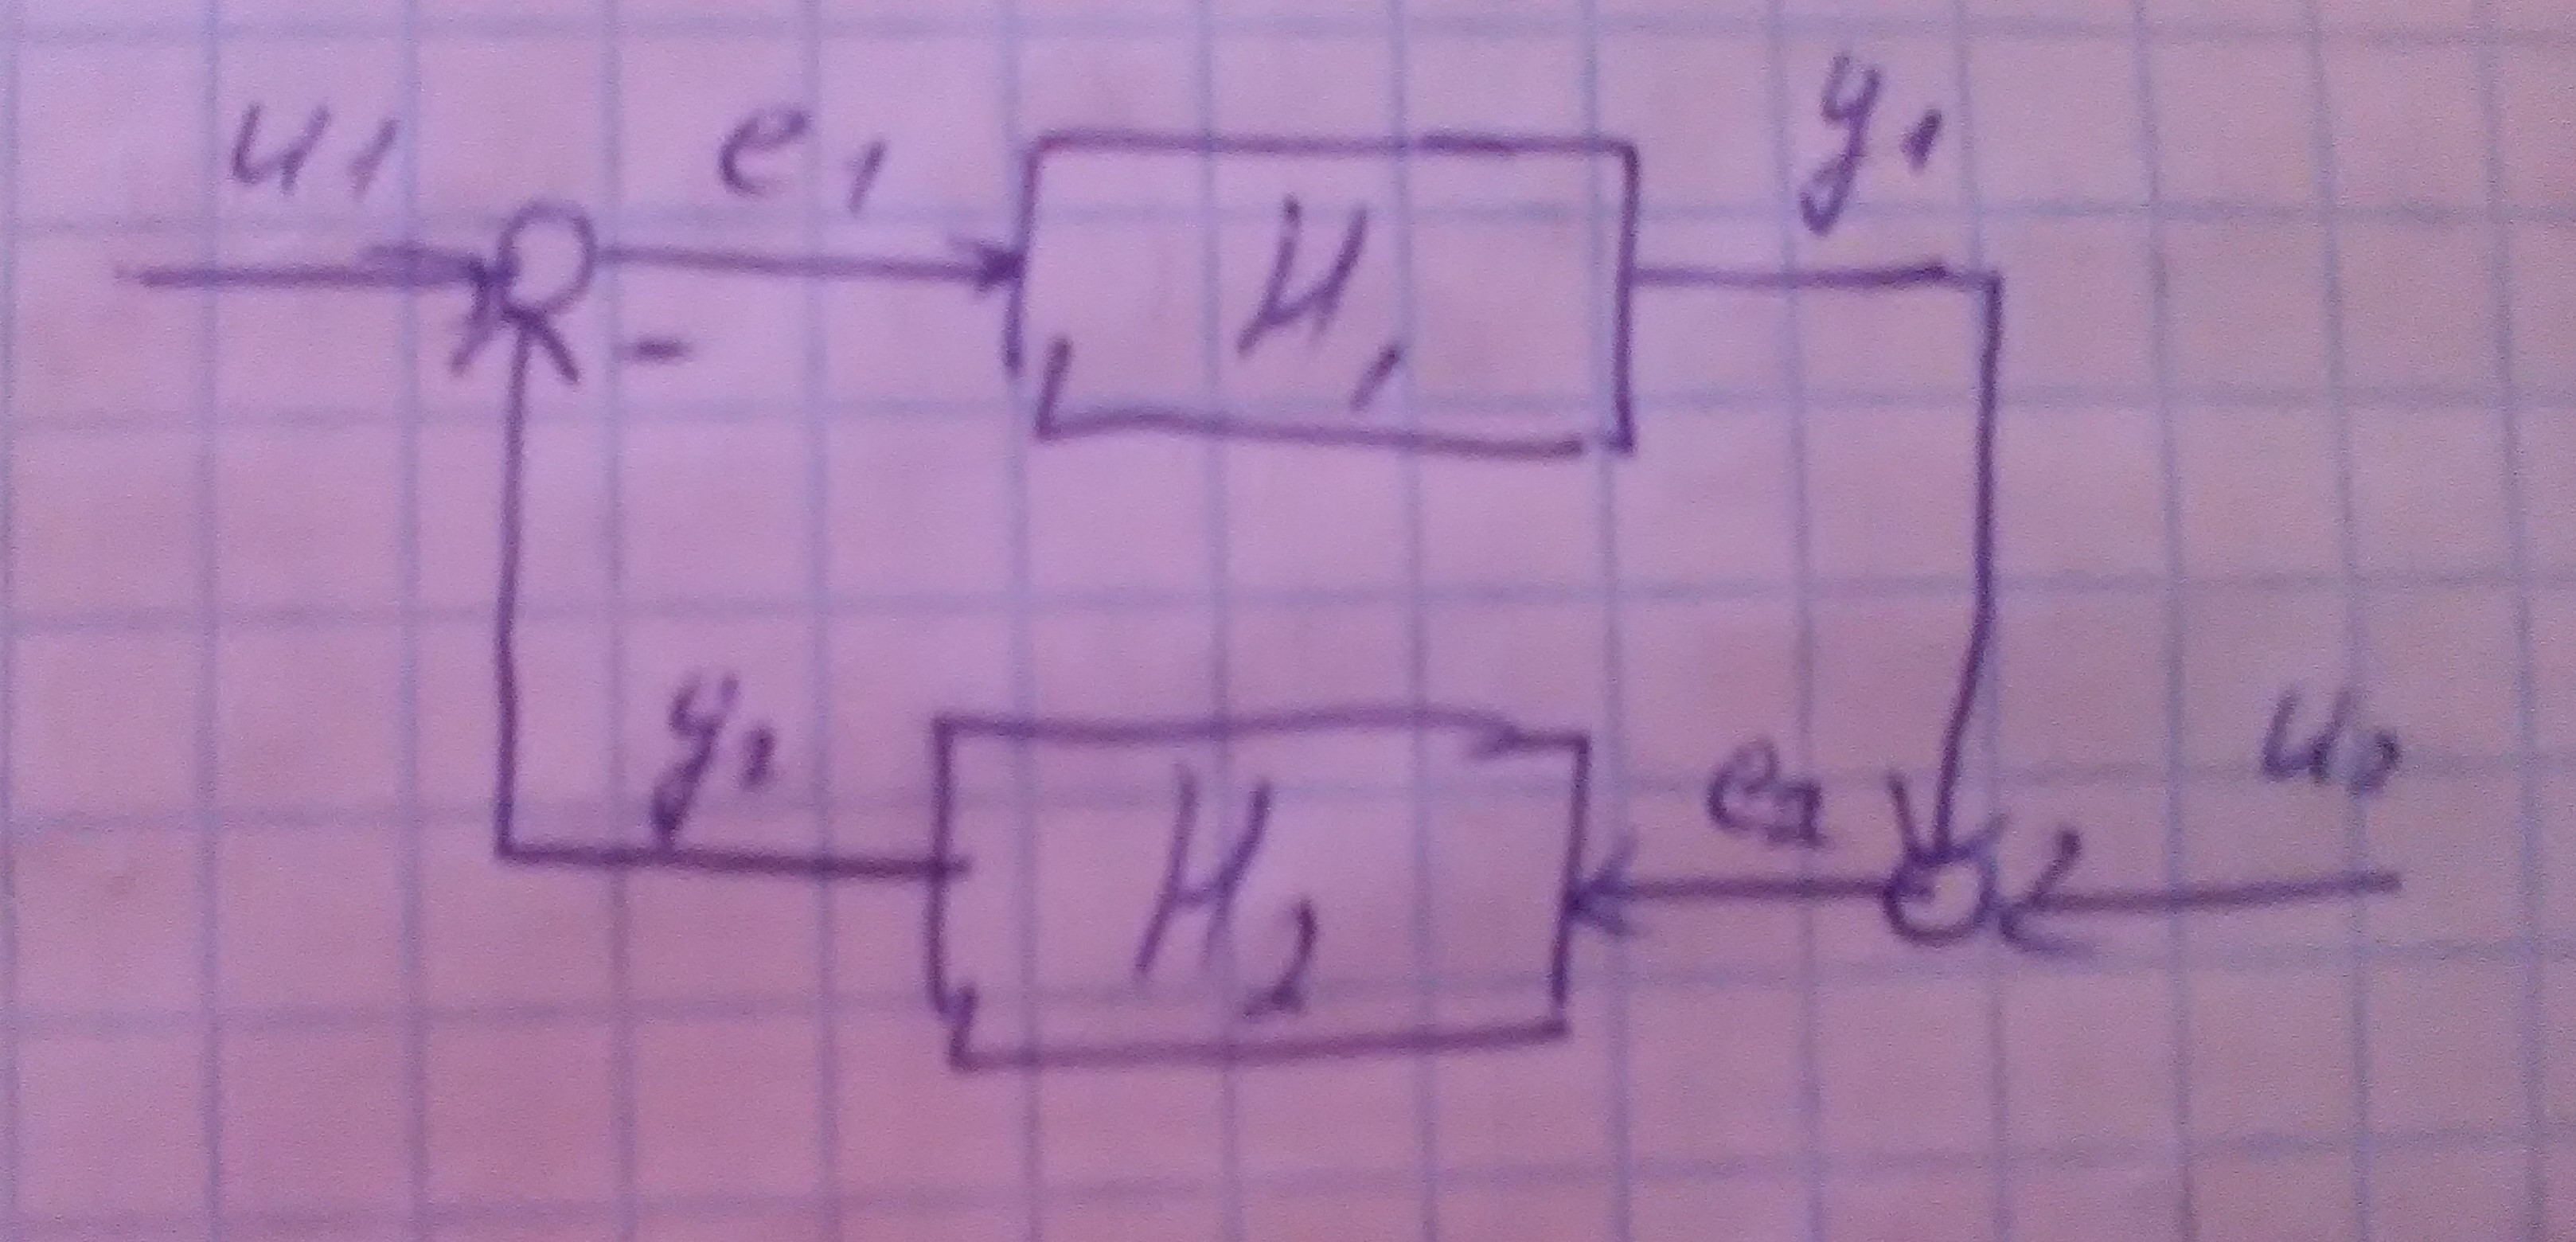
\includegraphics[scale=0.1]{5}
\end{center}

\begin{Theorem}
 Suppose that $H_1$ and $H_2$ are finite-gain $L_p$ stable (with gains $\gamma_1$, $\gamma_2$).
 Then the feedback interconnection is finite-gain $L_p$ stable if $\gamma_1\gamma_2<1$.

 \begin{proof}
   \begin{center}
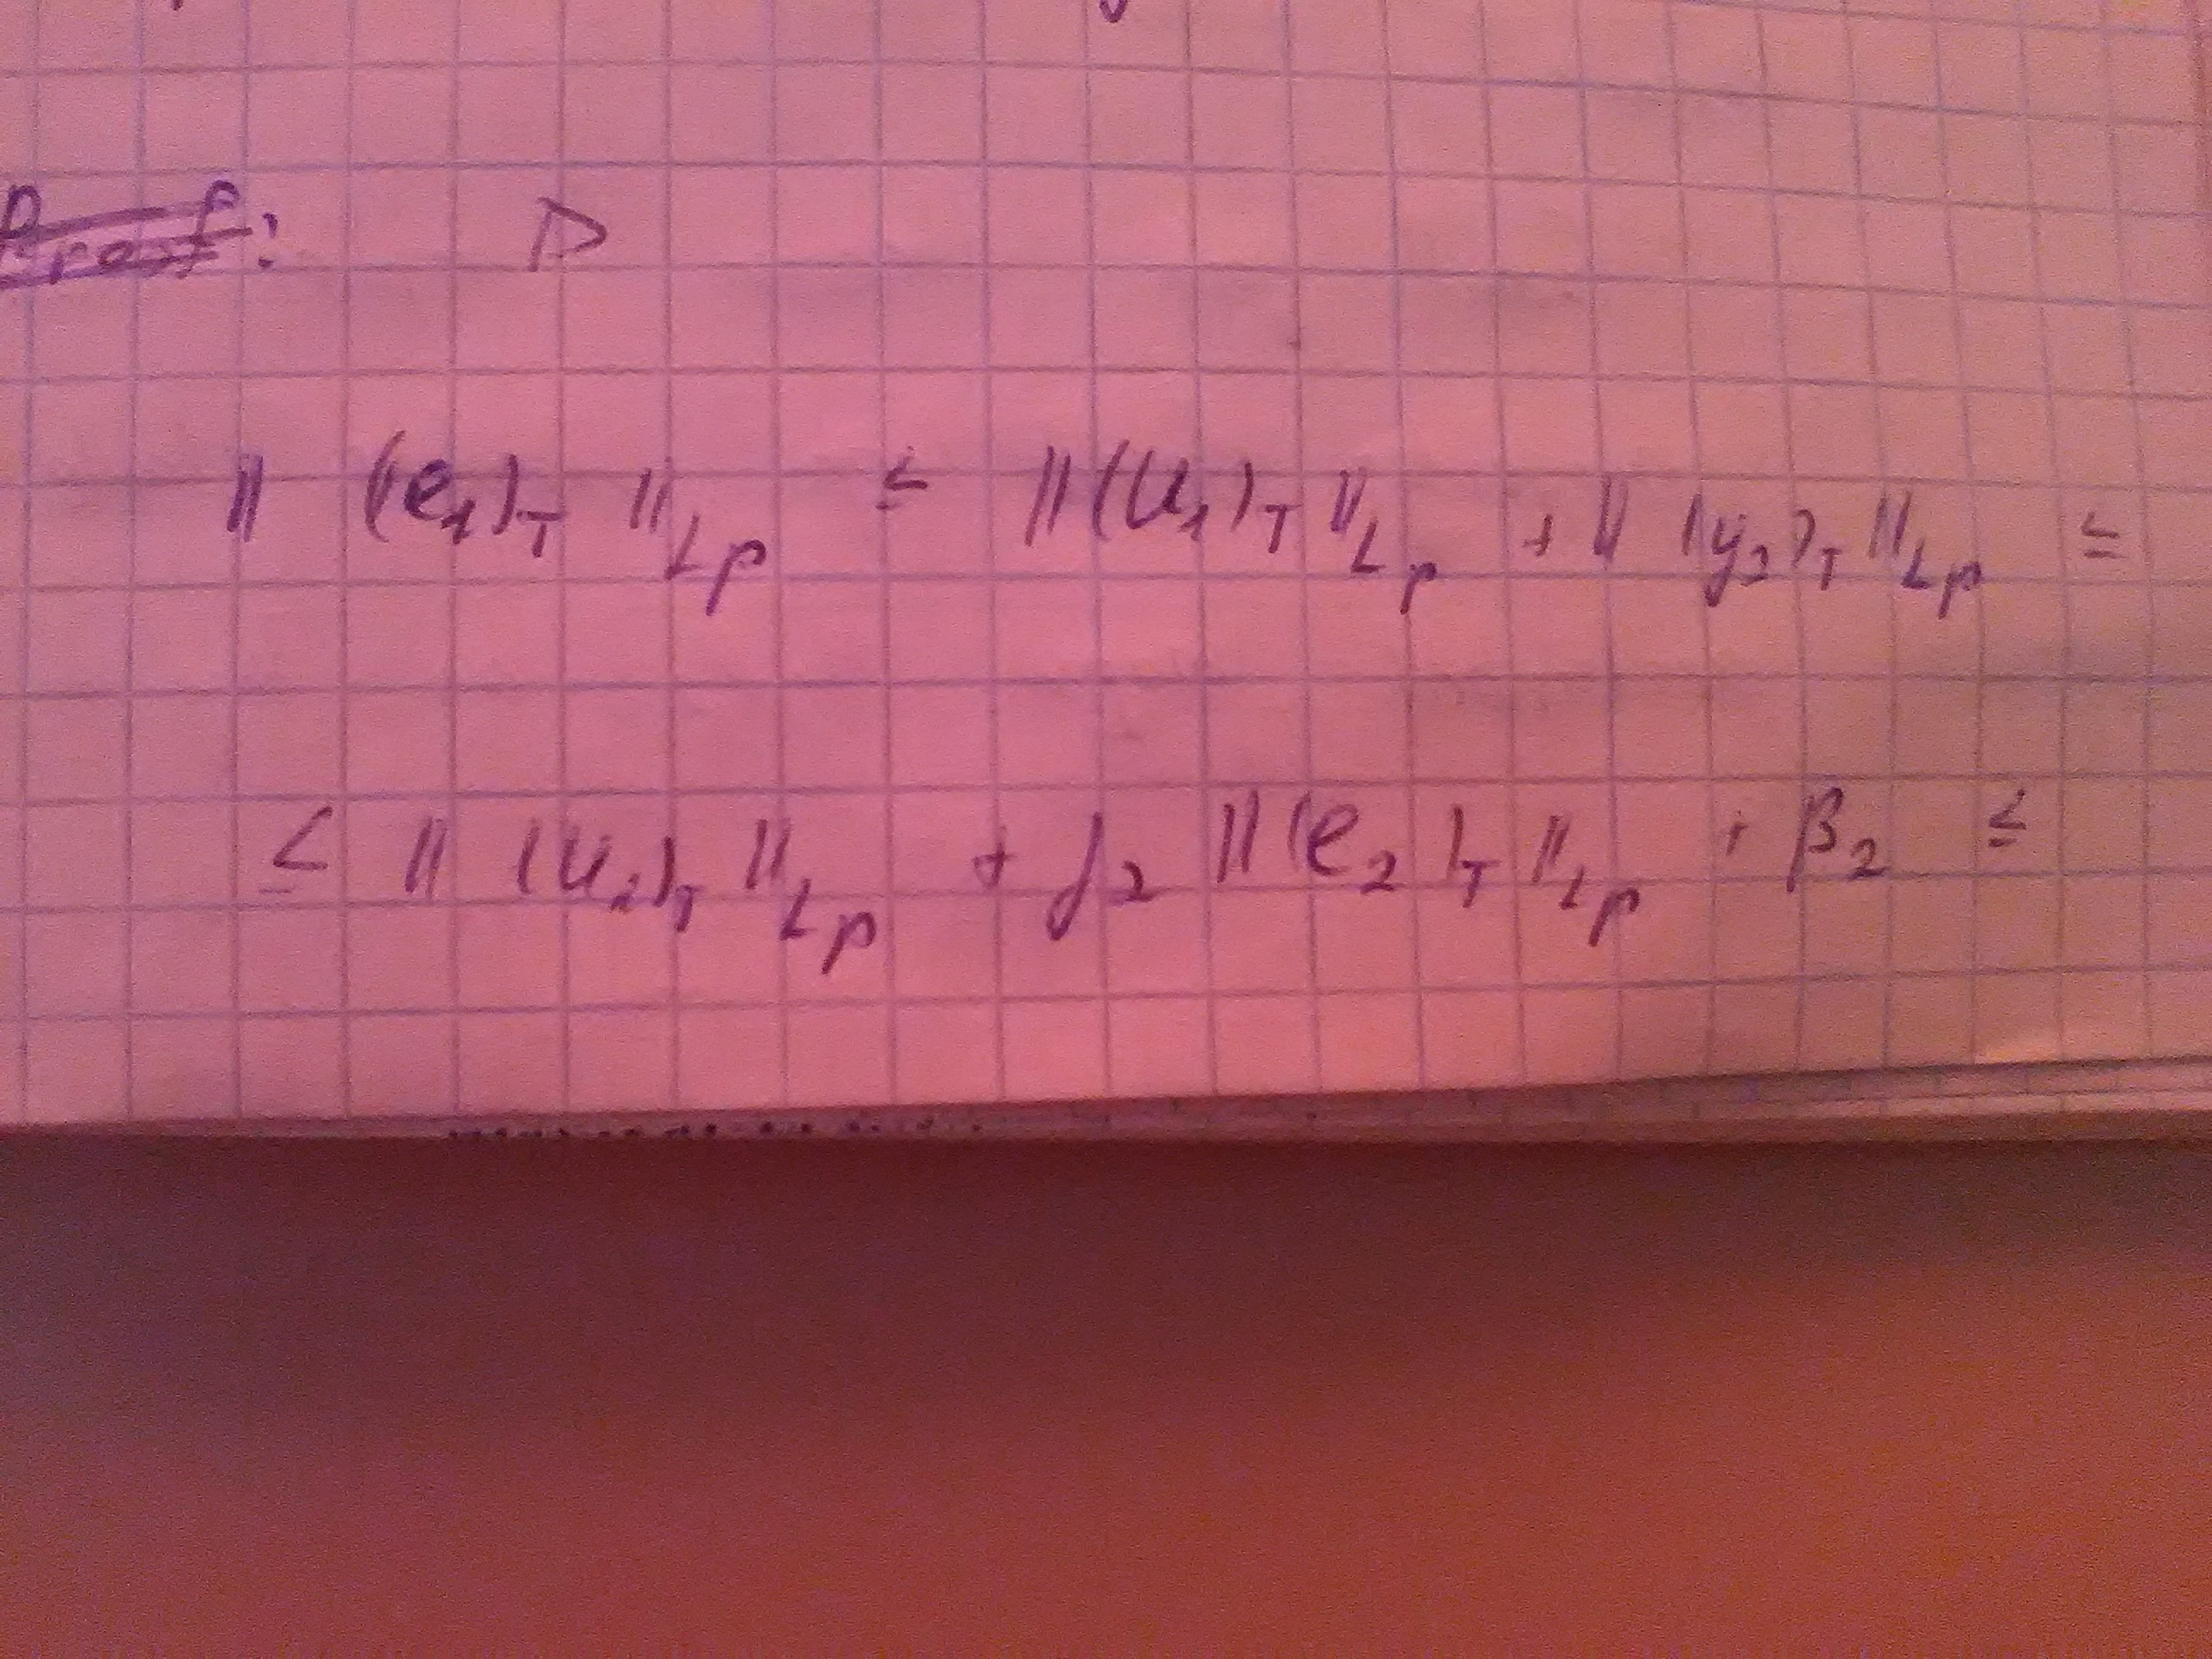
\includegraphics[scale=0.1]{13}
\end{center}
 \begin{center}
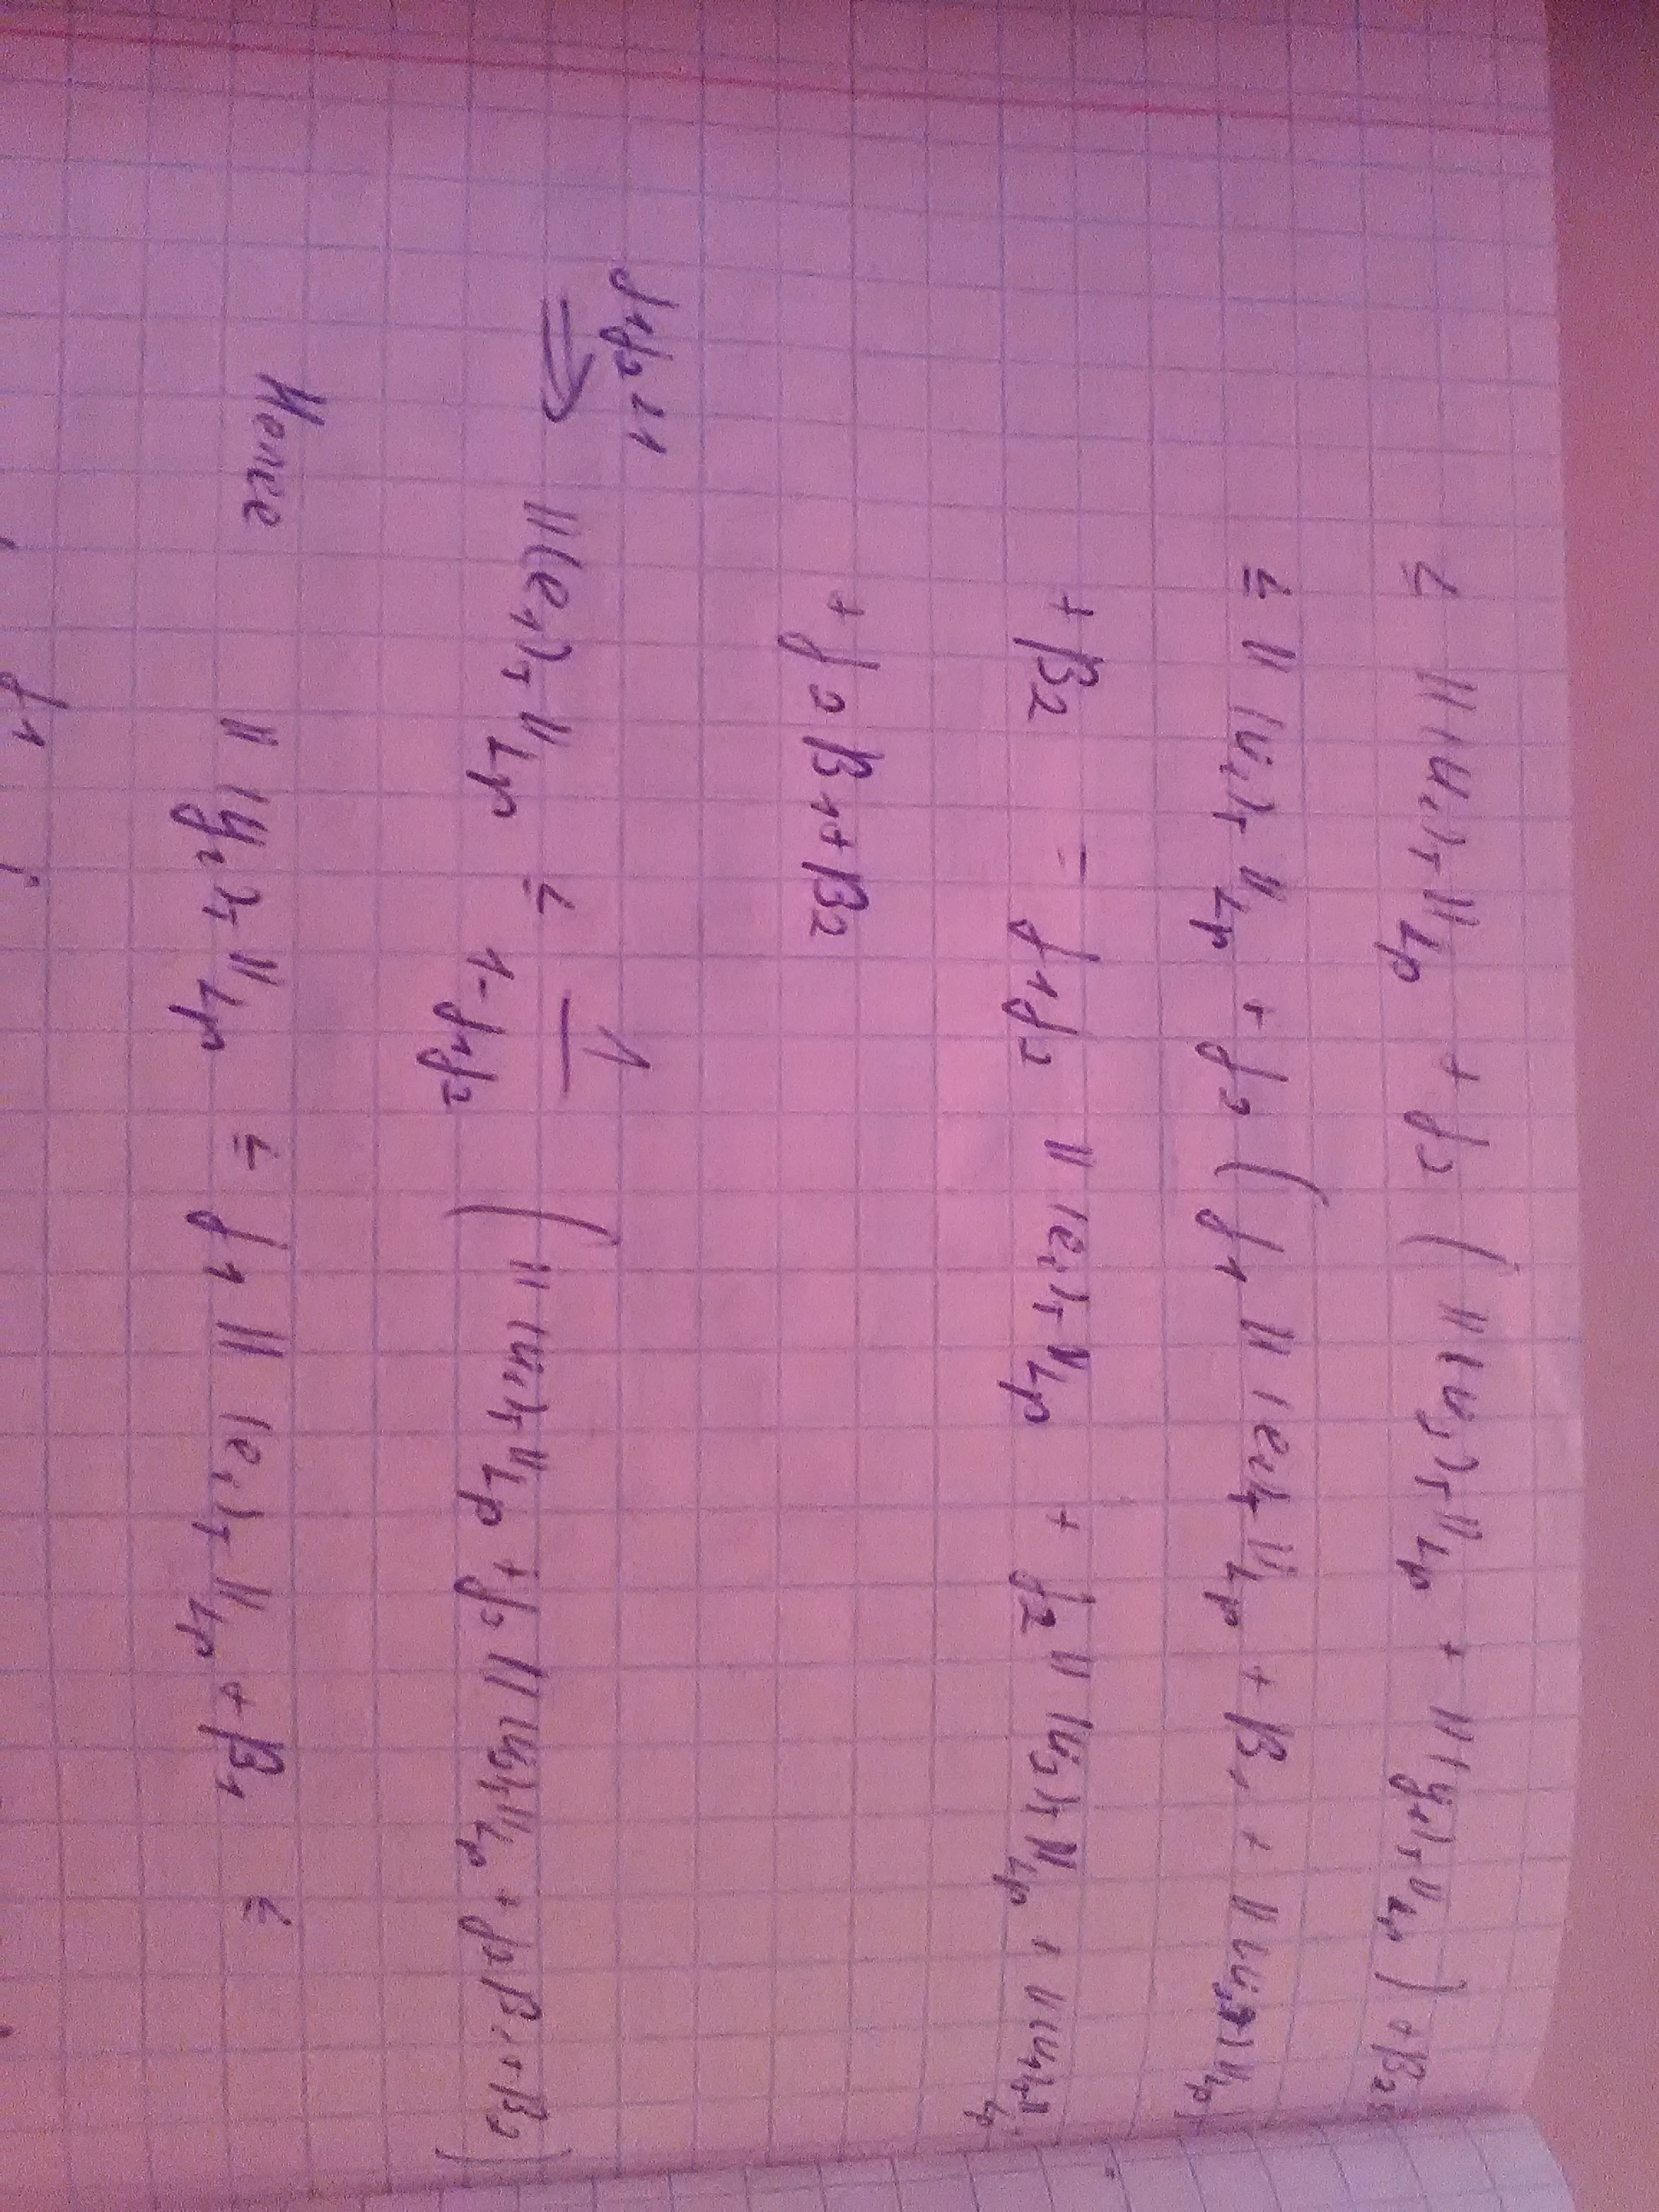
\includegraphics[scale=0.1]{14}
\end{center}
 \begin{center}
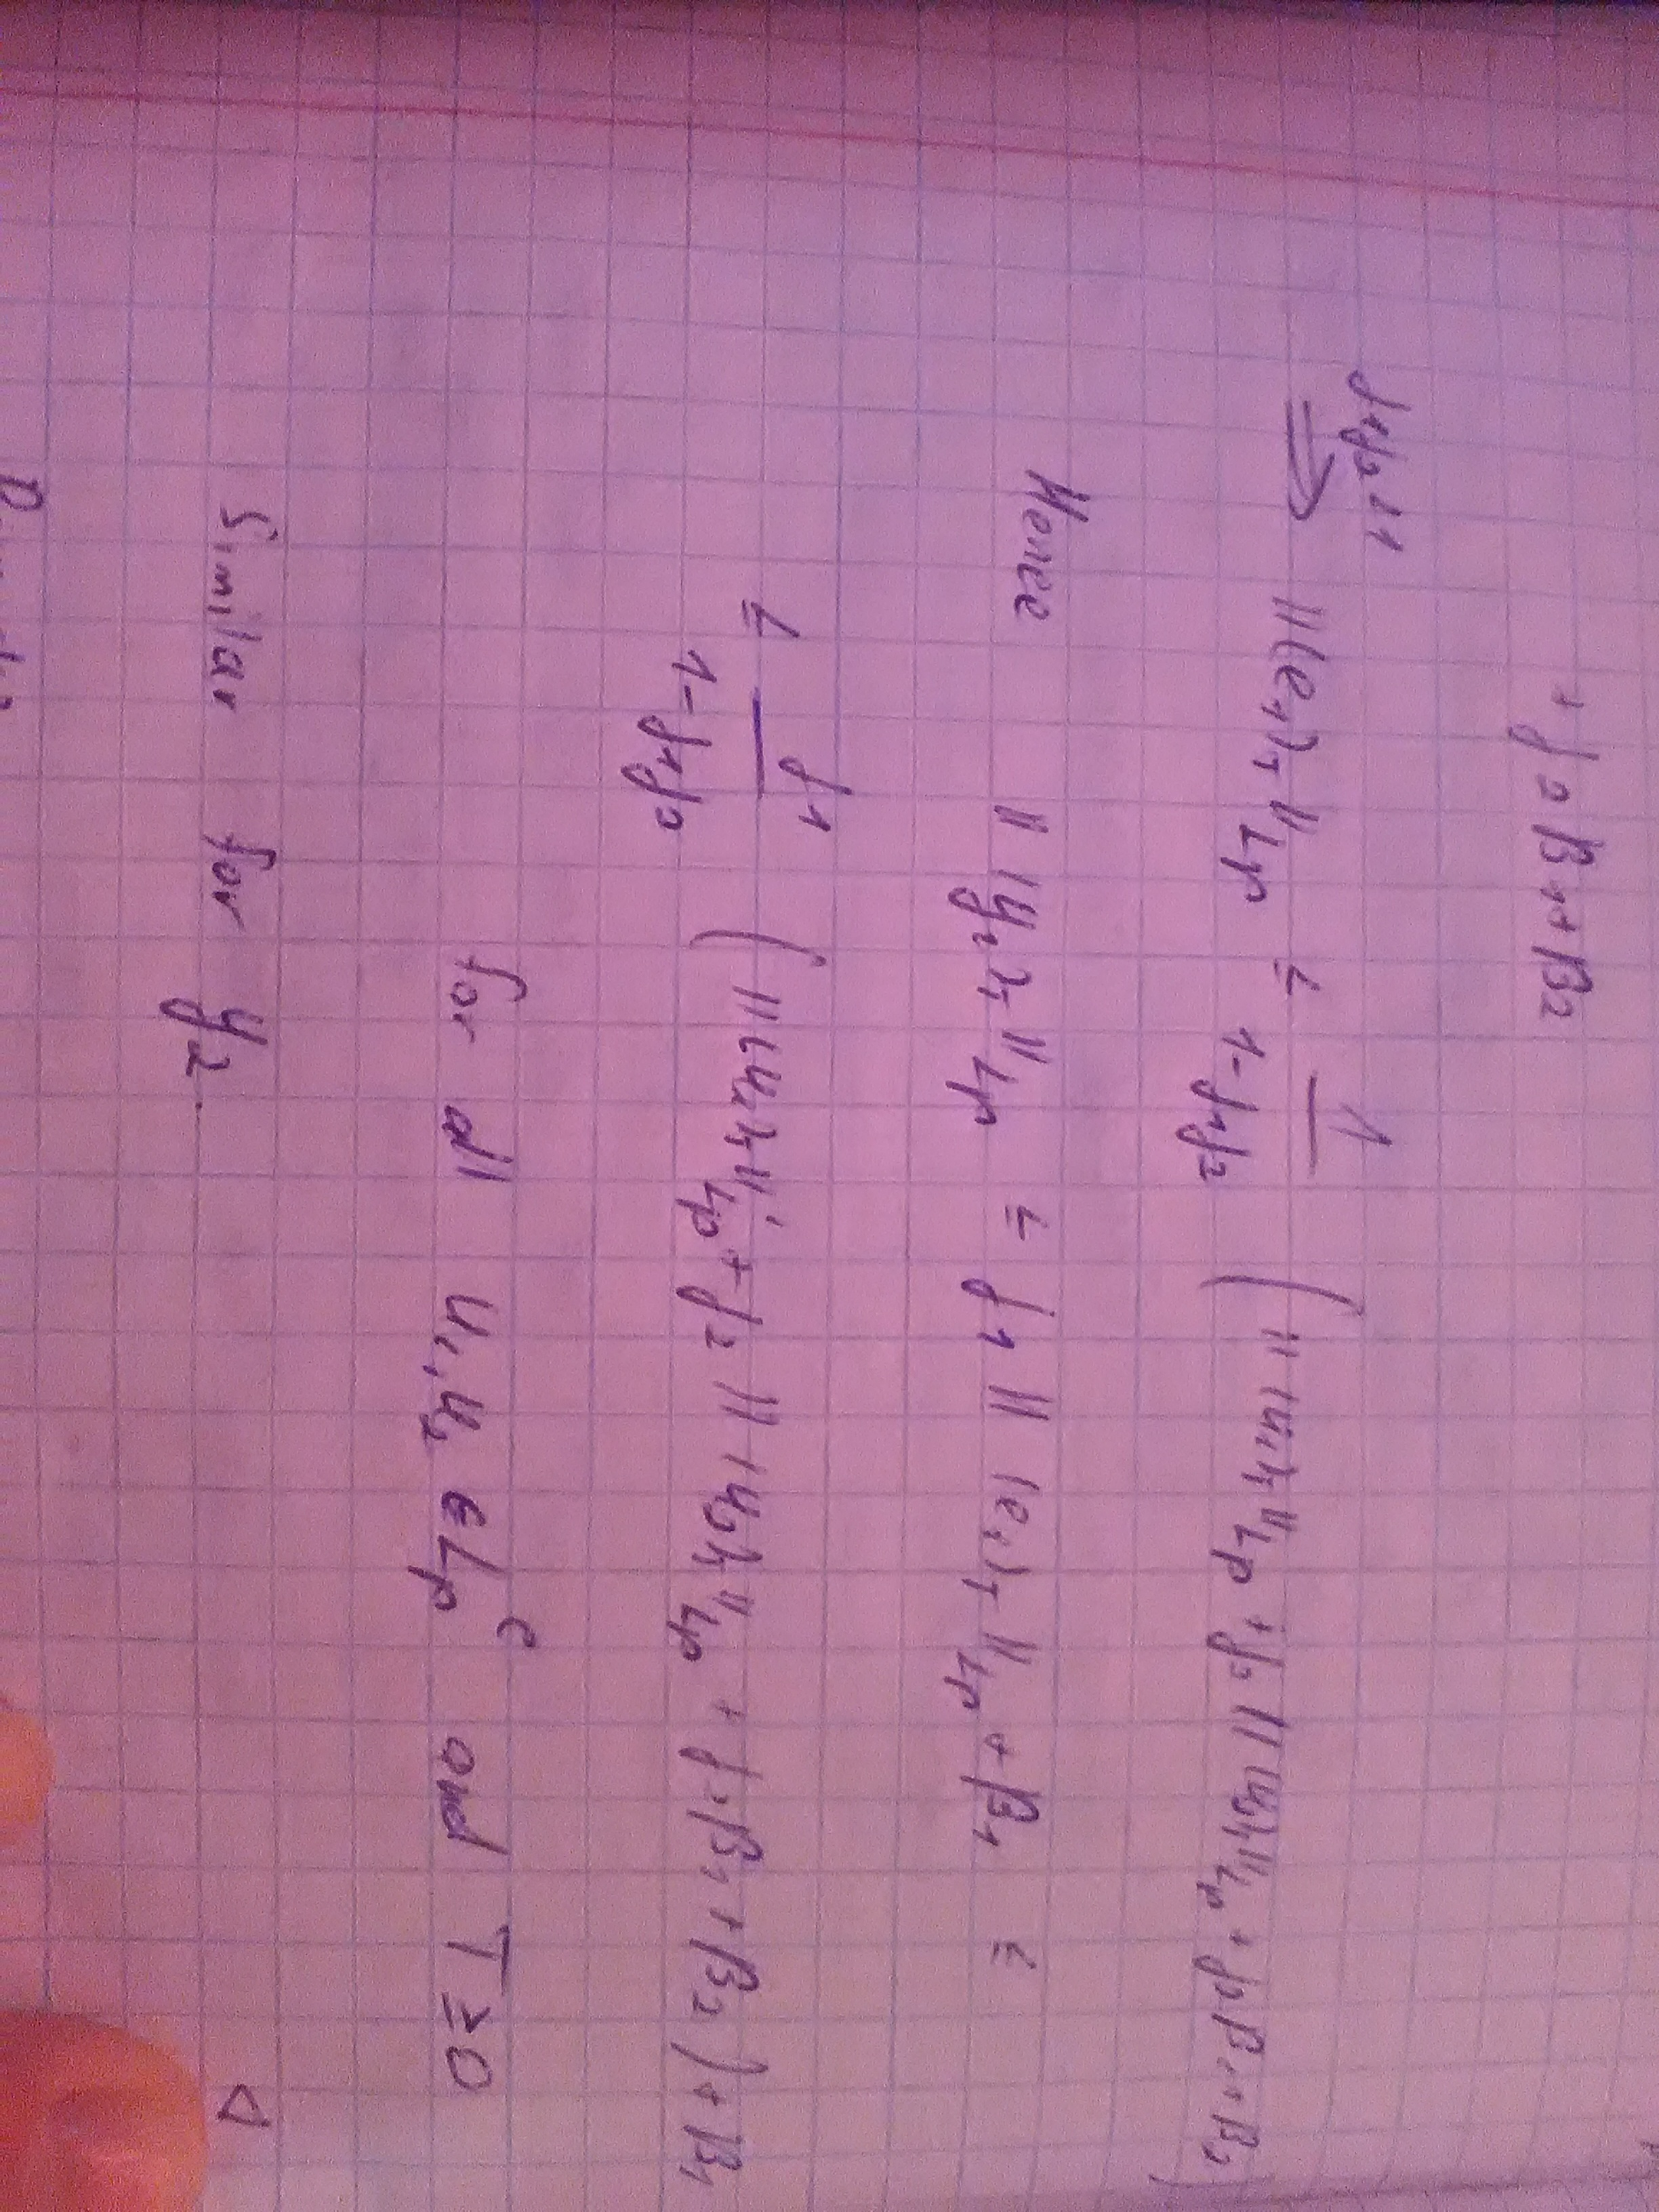
\includegraphics[scale=0.1]{15}
\end{center}
 \end{proof}
\end{Theorem}

Remark: Small gain theorem implies inherent robastness property: closed loop remains stable
for perturbed maps $H_1$, $H_2$ as long as $\gamma_1\gamma_2<1$.

Example:

 \begin{center}
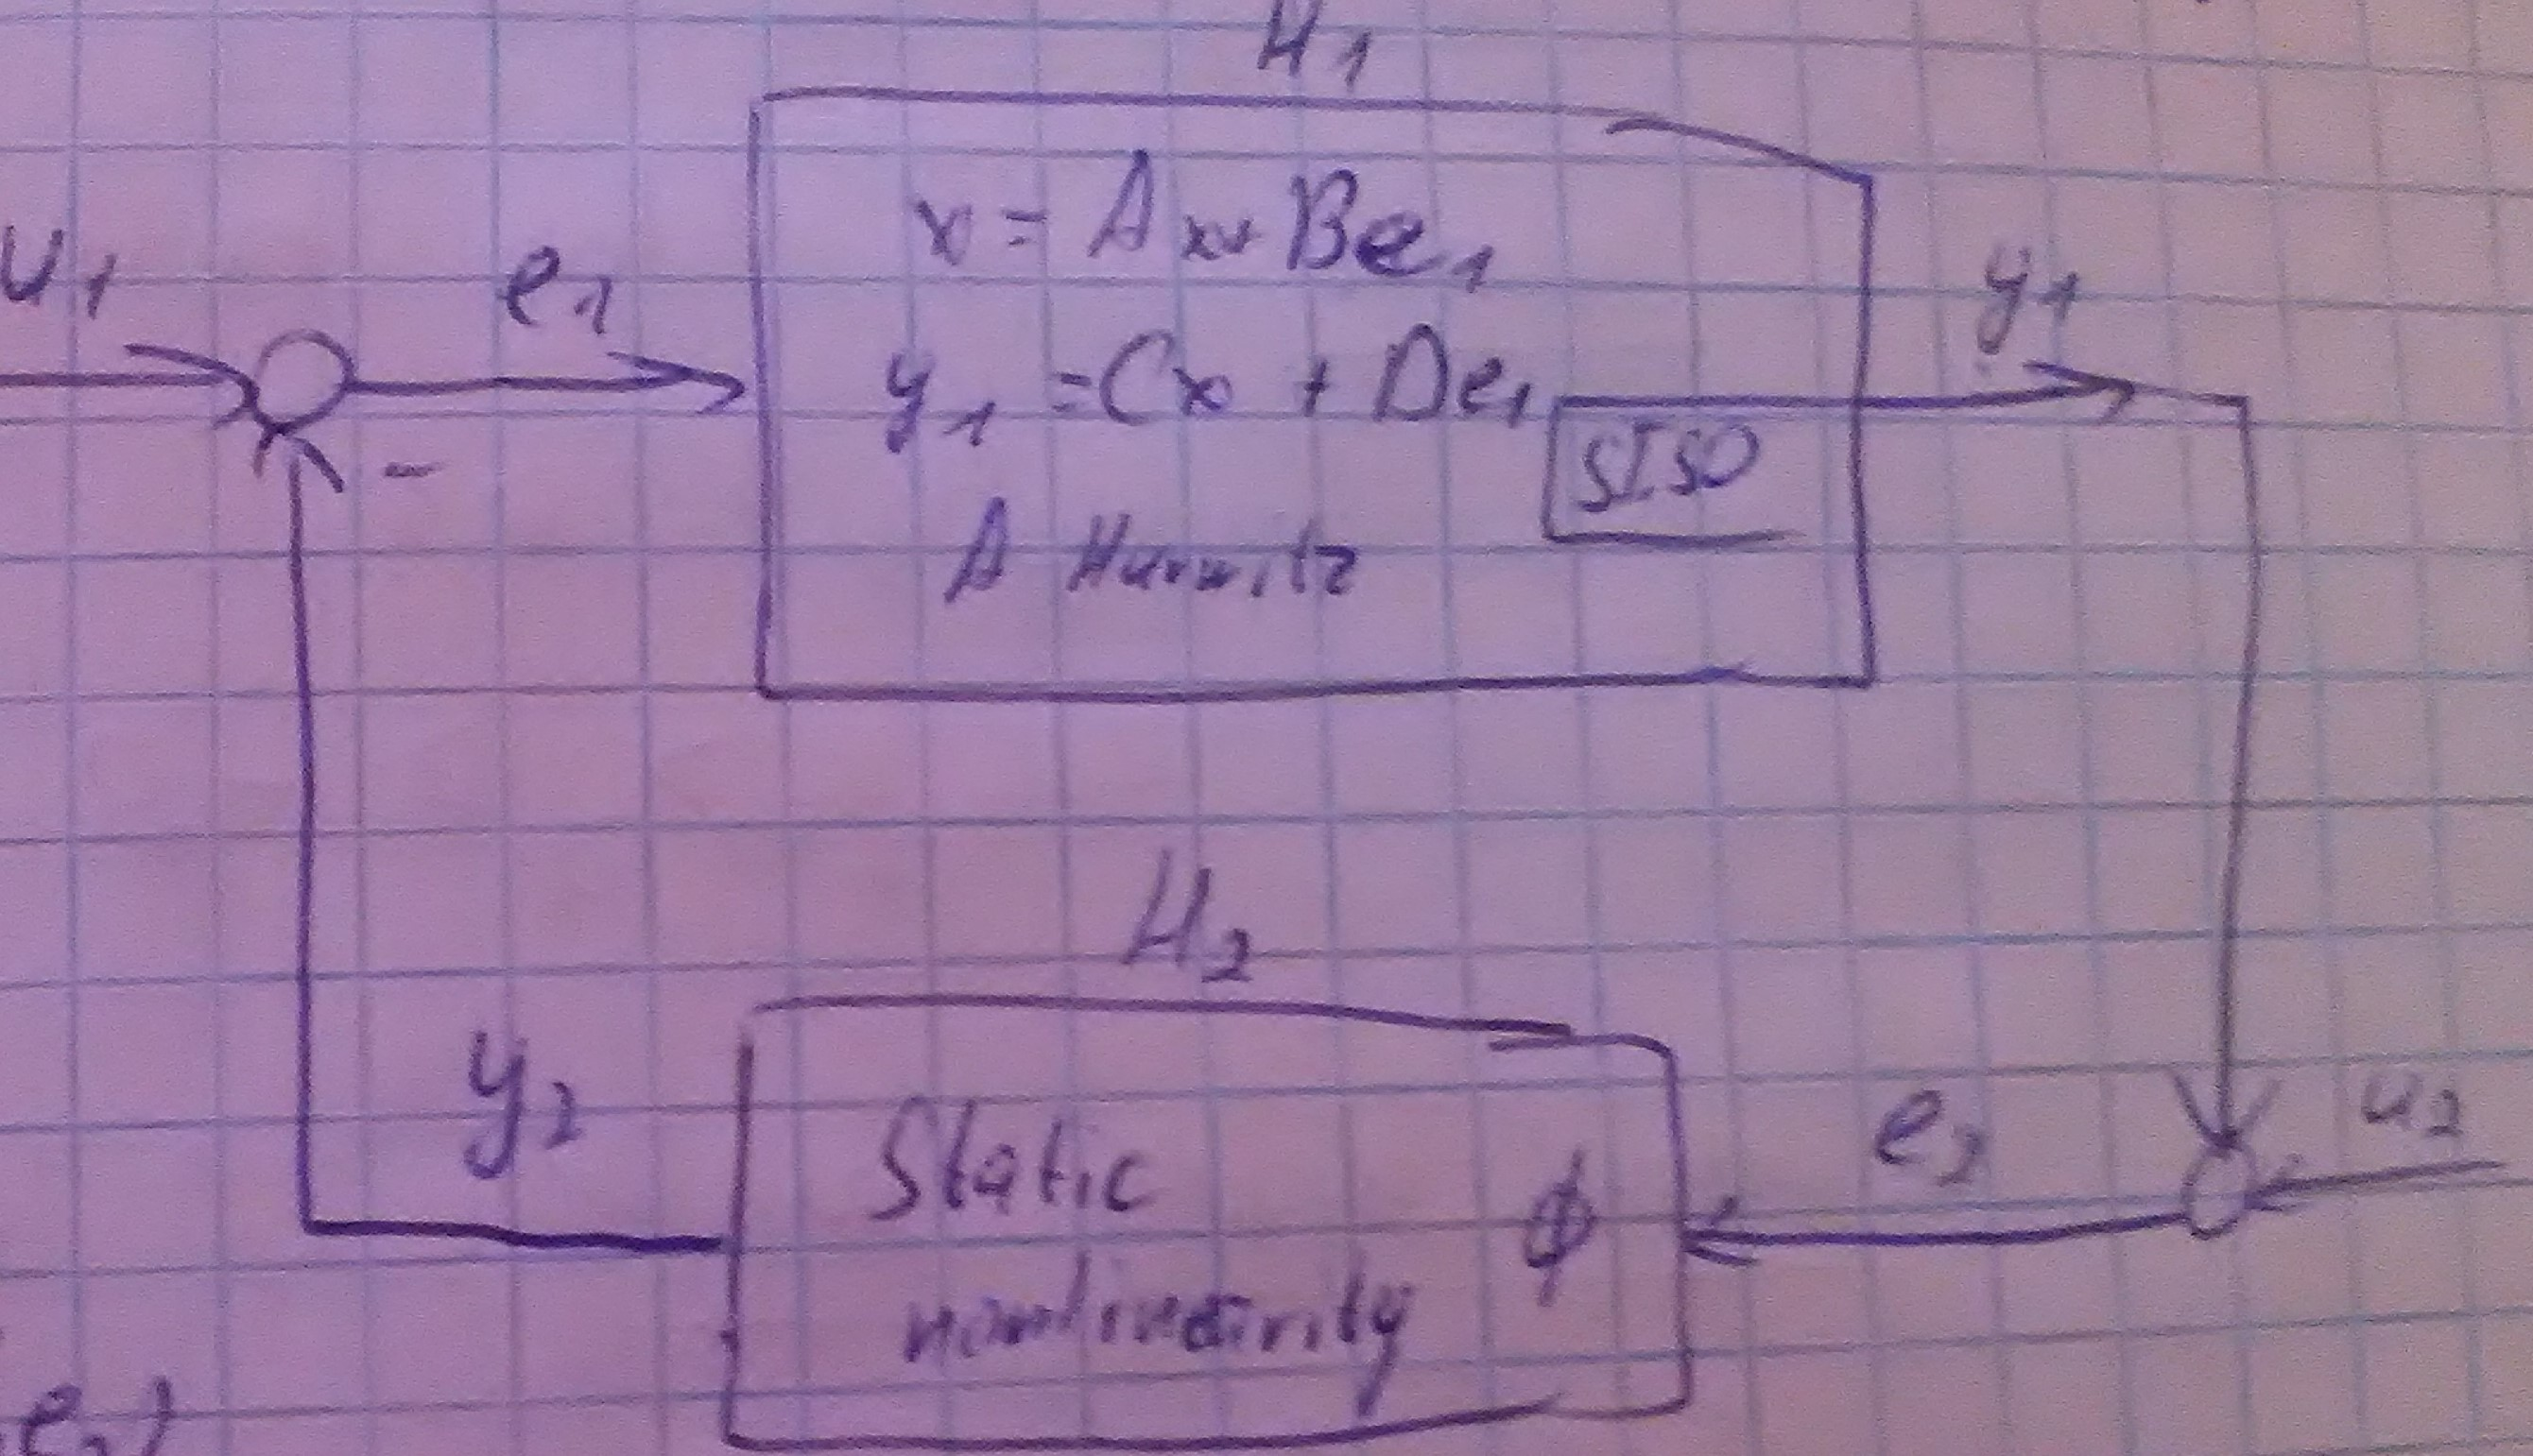
\includegraphics[scale=0.1]{6}
\end{center}

\begin{equation}
H_1:
\begin{split}
 &x=Ax+Be_1\\
 &y_1=Cx+De_1\\
 &A\ is\ Hurwitz
\end{split}
\end{equation}


\begin{equation}
H_2: y=\Phi(t,e_2)
\end{equation}

We know, that $H_1$ has gain $\gamma_1=\sup_{w\in\mathbb{R}}\sqrt{G(-jw)G(jw)}$.

Suppose: $|\Phi(t,e_2)|\le\gamma_2|e_2|$, $\forall t\ge0$, $\forall e_2\in\mathbb{R}$
$\Rightarrow$ $H_2$ has $L_2$ gain $\le\gamma_2$.

Passivity framework ($p=2$)

\begin{Definition}
 $H:L_p^e\rightarrow L_p^e$ is

 {\it passive} if there exist $B\in\mathbb{R}$ s.t. $\forall u\in L_p^e$, $\forall T\ge0$,
 $<u_T,y^T>\ \ge -B$

 {\it output-strictly passive} if there exists $B\in\mathbb{R}$ and $\epsilon>0$ s.t.
 $\forall u\in L_p^e$, $\forall T\ge0$ follows  $<u_T,y^T>\ \ge -B+\epsilon ||y_T||_{L_2}^2$
\end{Definition}

\begin{Lemma}
 Let $H:L_p^e\rightarrow L_p^e$ be output strictly passive with excess $\epsilon$. Then $H$
 has $L_2$-gain $\le\frac{1}{\epsilon}$.
 \begin{proof}
	 \begin{center}
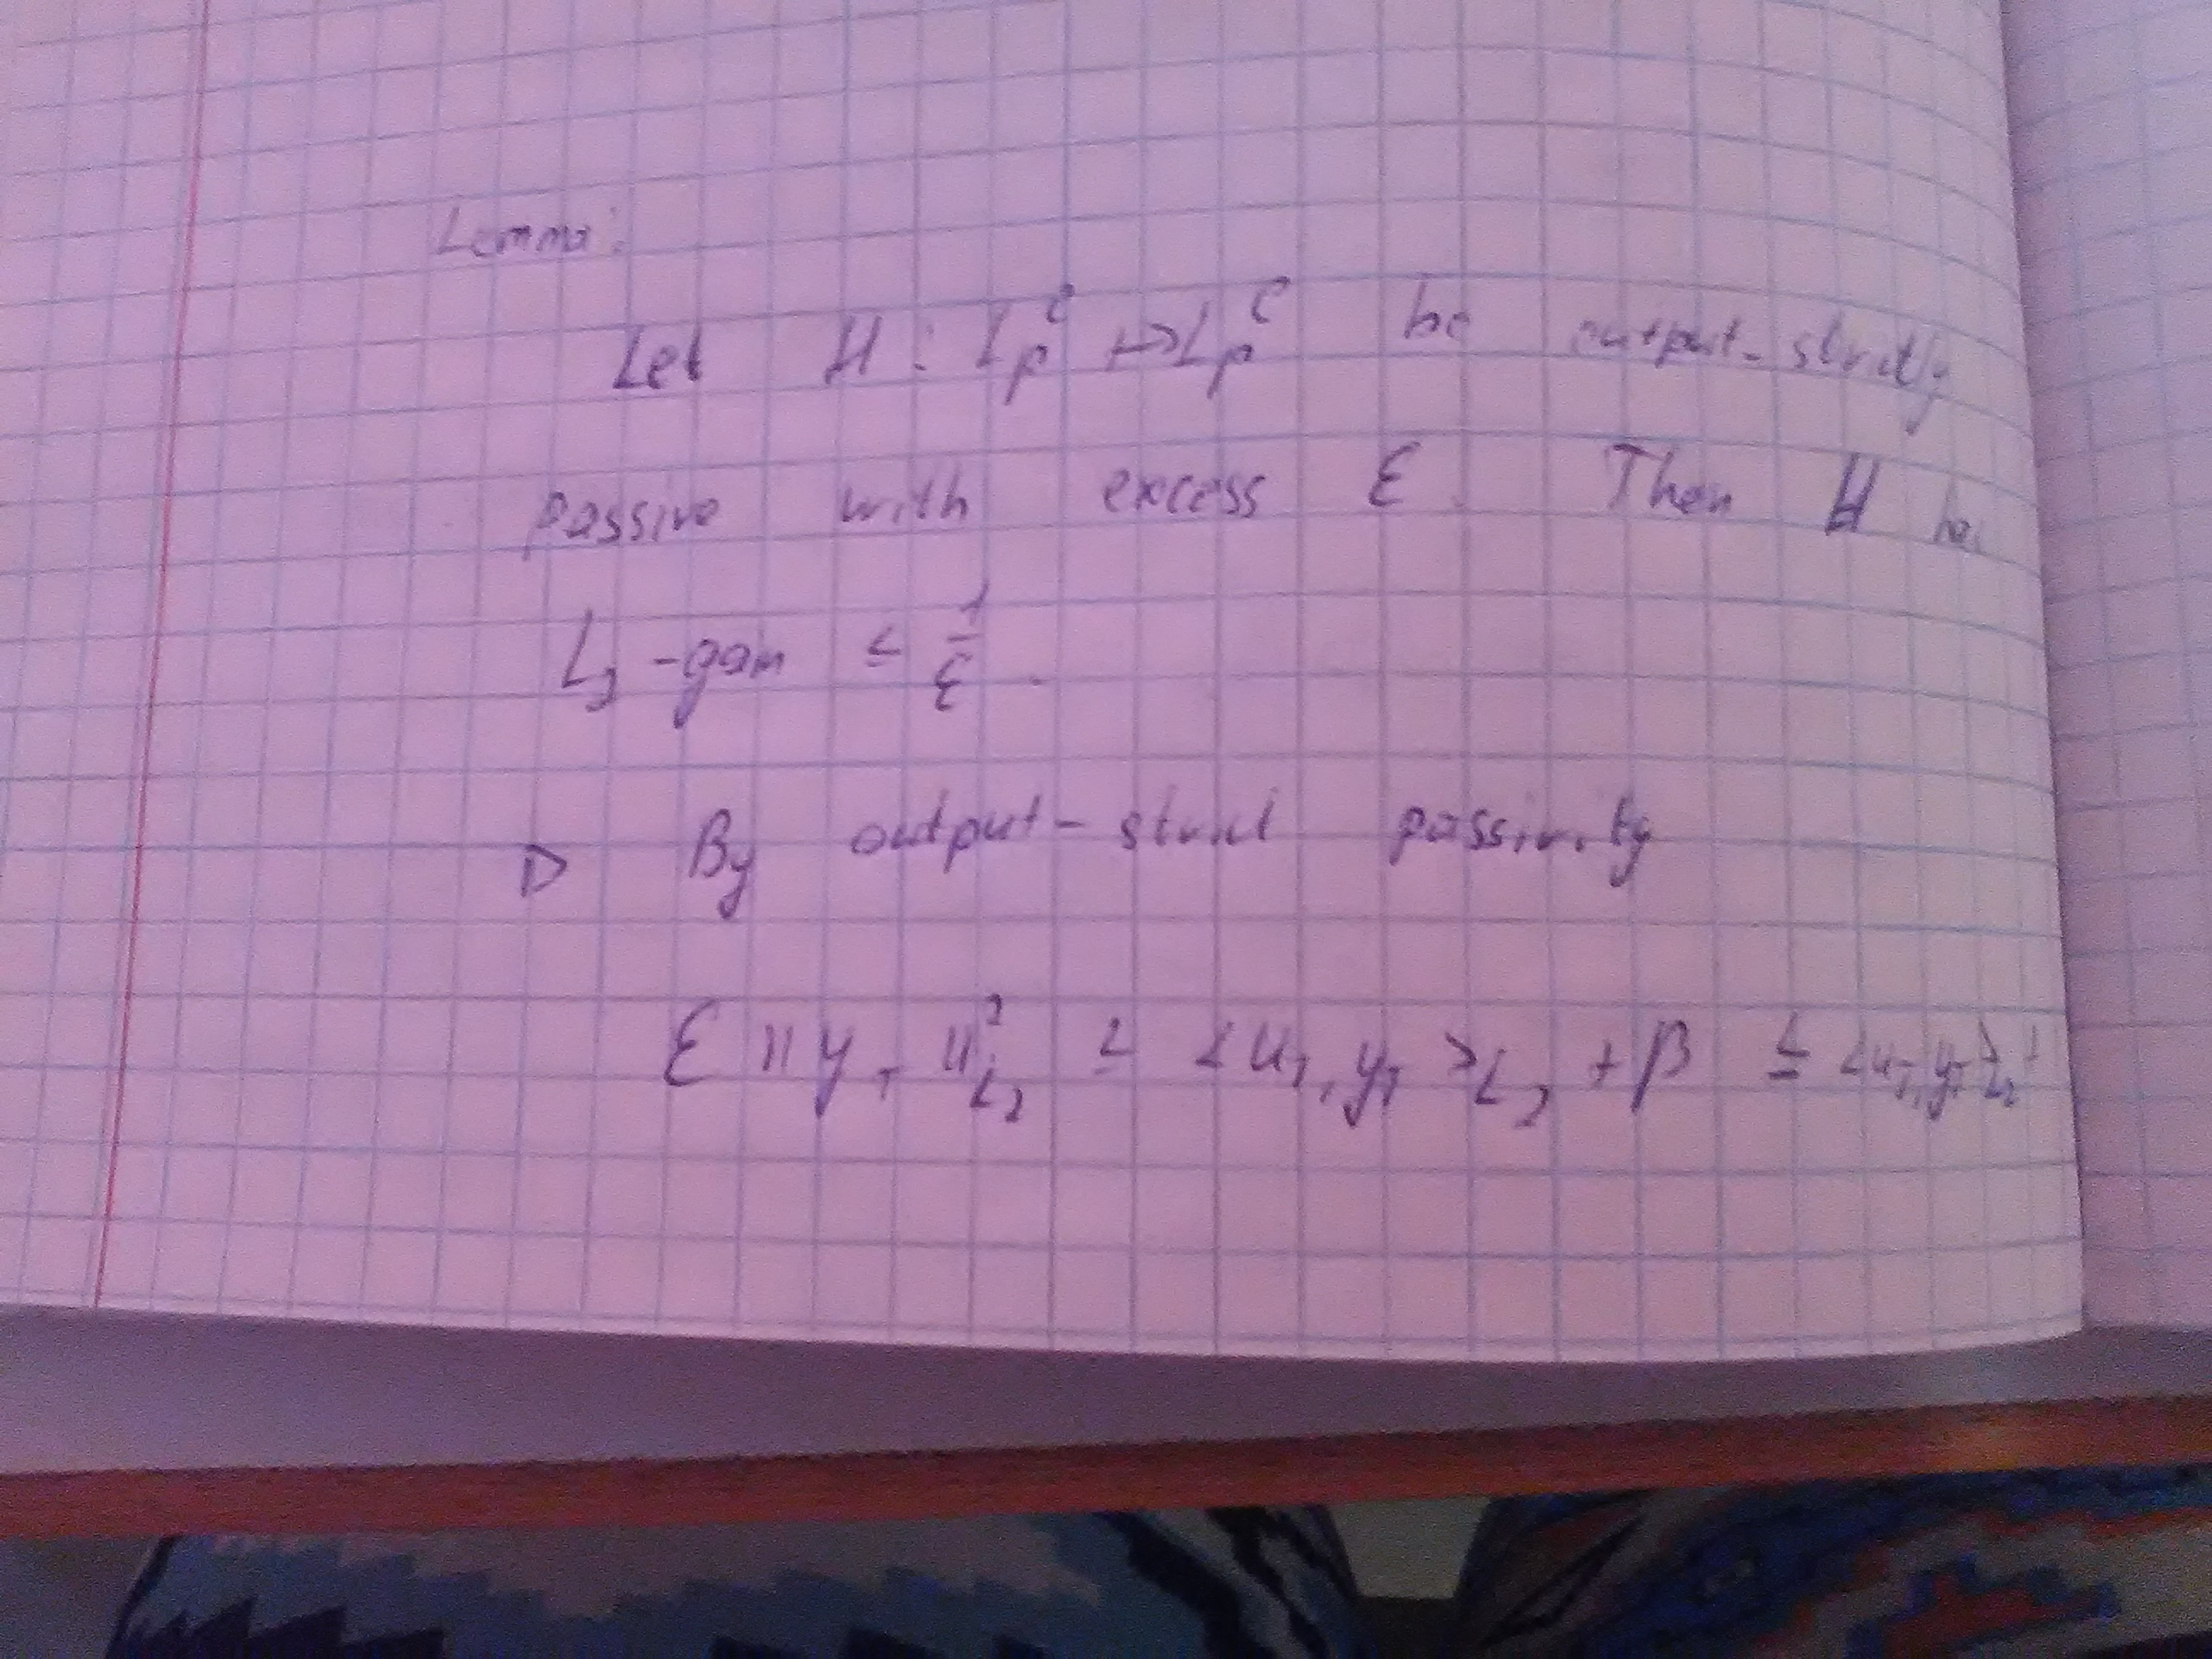
\includegraphics[scale=0.1]{7}
\end{center}
 \begin{center}
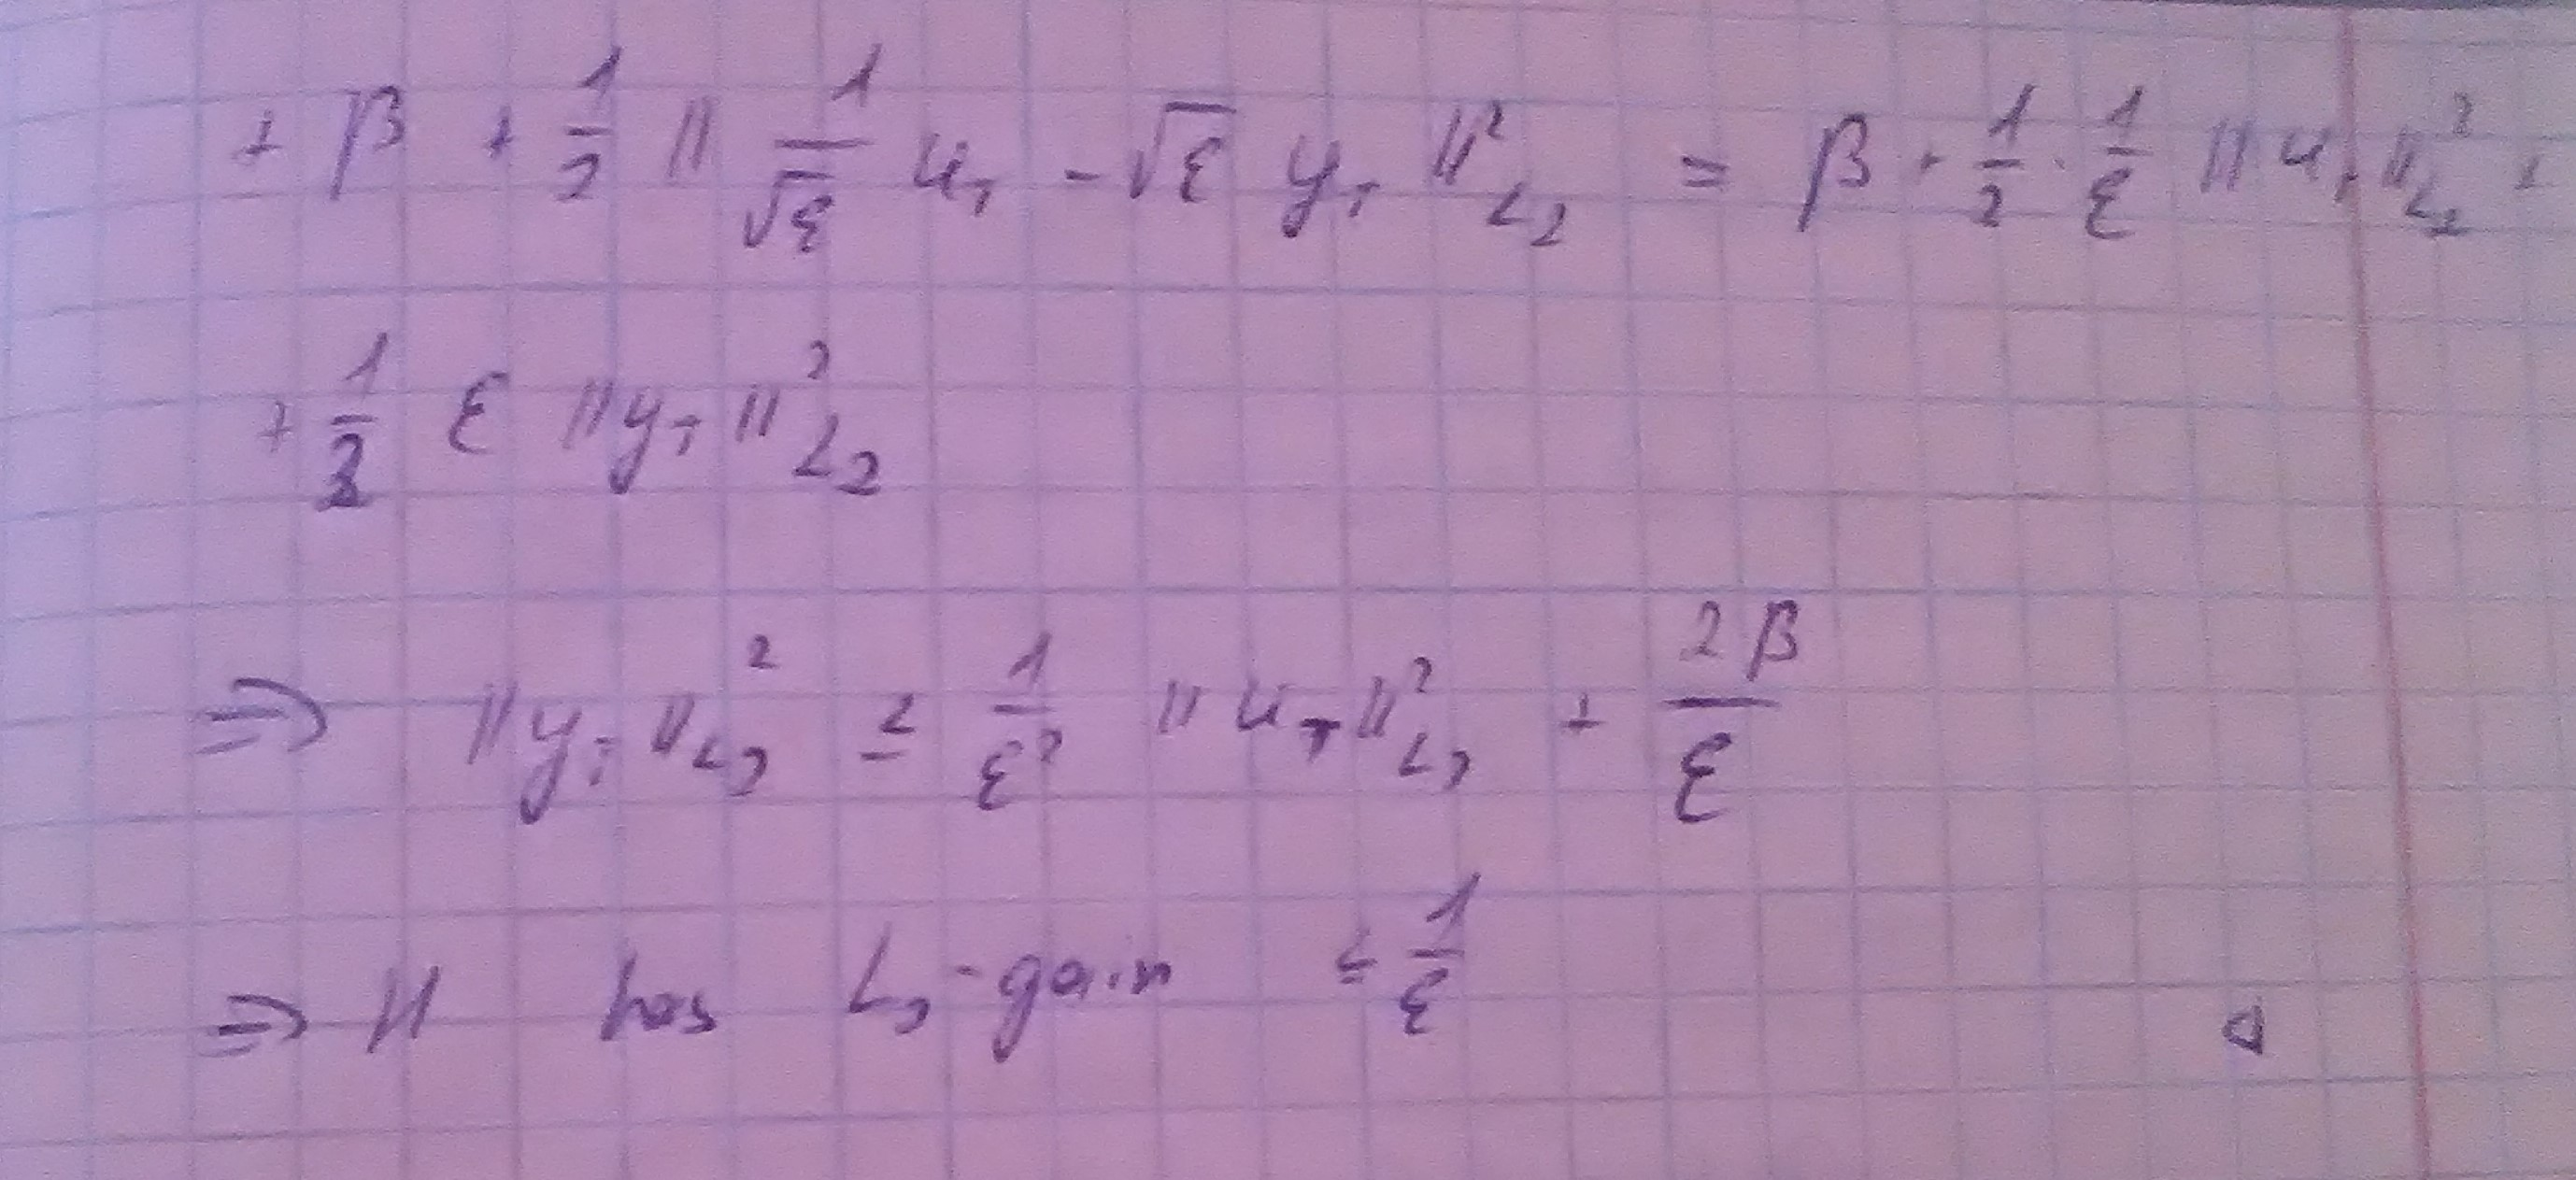
\includegraphics[scale=0.1]{8}
\end{center}
\end{proof}	
\end{Lemma}

\begin{Theorem}[Feedback theorem for passive system in I/O framework]
 Suppose there exist $\epsilon_i, \delta_i, \beta_i$; $i=1,2$ s.t.

 $$<(e_i)_T, (H_i(e_i))_T>_{L_2} \ge \epsilon_i ||(H_i(e_i))_T||_{L_2}^2+\delta_i
 ||(e_i)_T||_{L_2}^2-\beta_i$$

 for all $T\ge0, \ e_i\in L_2^e$, $i=1,2$. If $\epsilon_1+\delta_2>0$ and $\epsilon_2+\delta_1>0$
 then the feedback interconnection has finite $L_2$-gain from $(u_1,u_2)\rightarrow(y_1,y_2)$.
 \begin{proof}
   \begin{center}
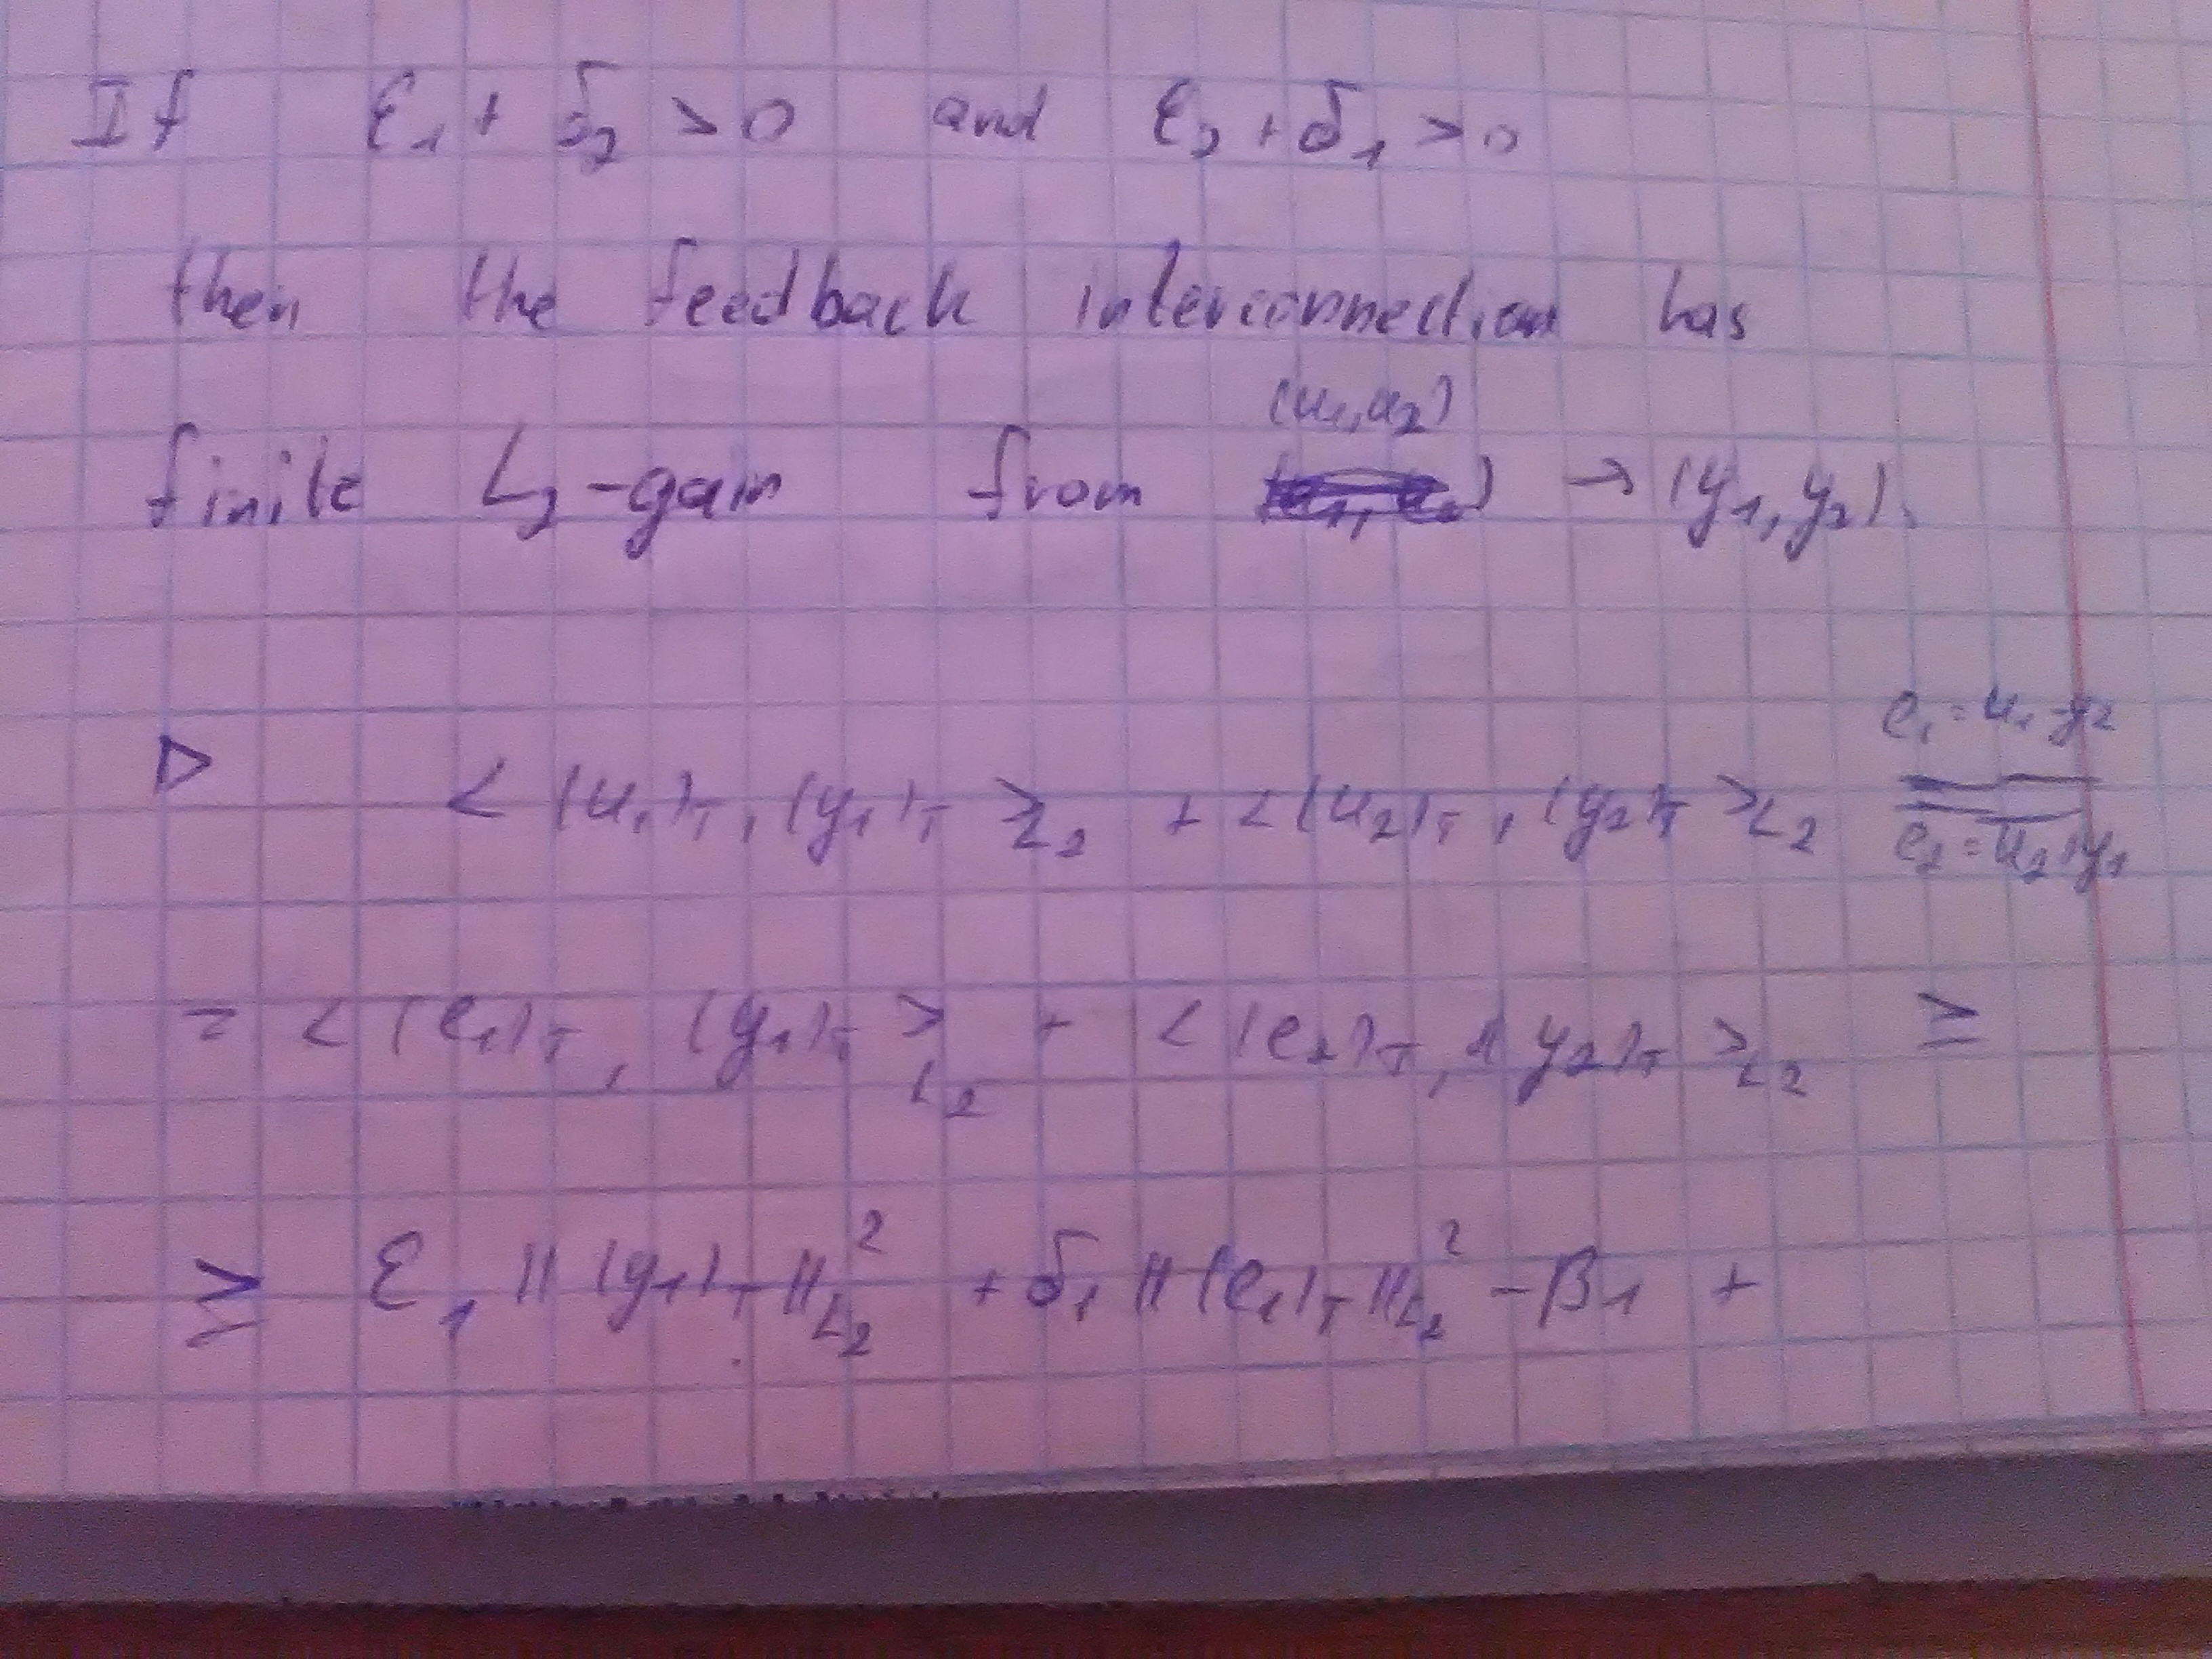
\includegraphics[scale=0.1]{9}
\end{center}
 \begin{center}
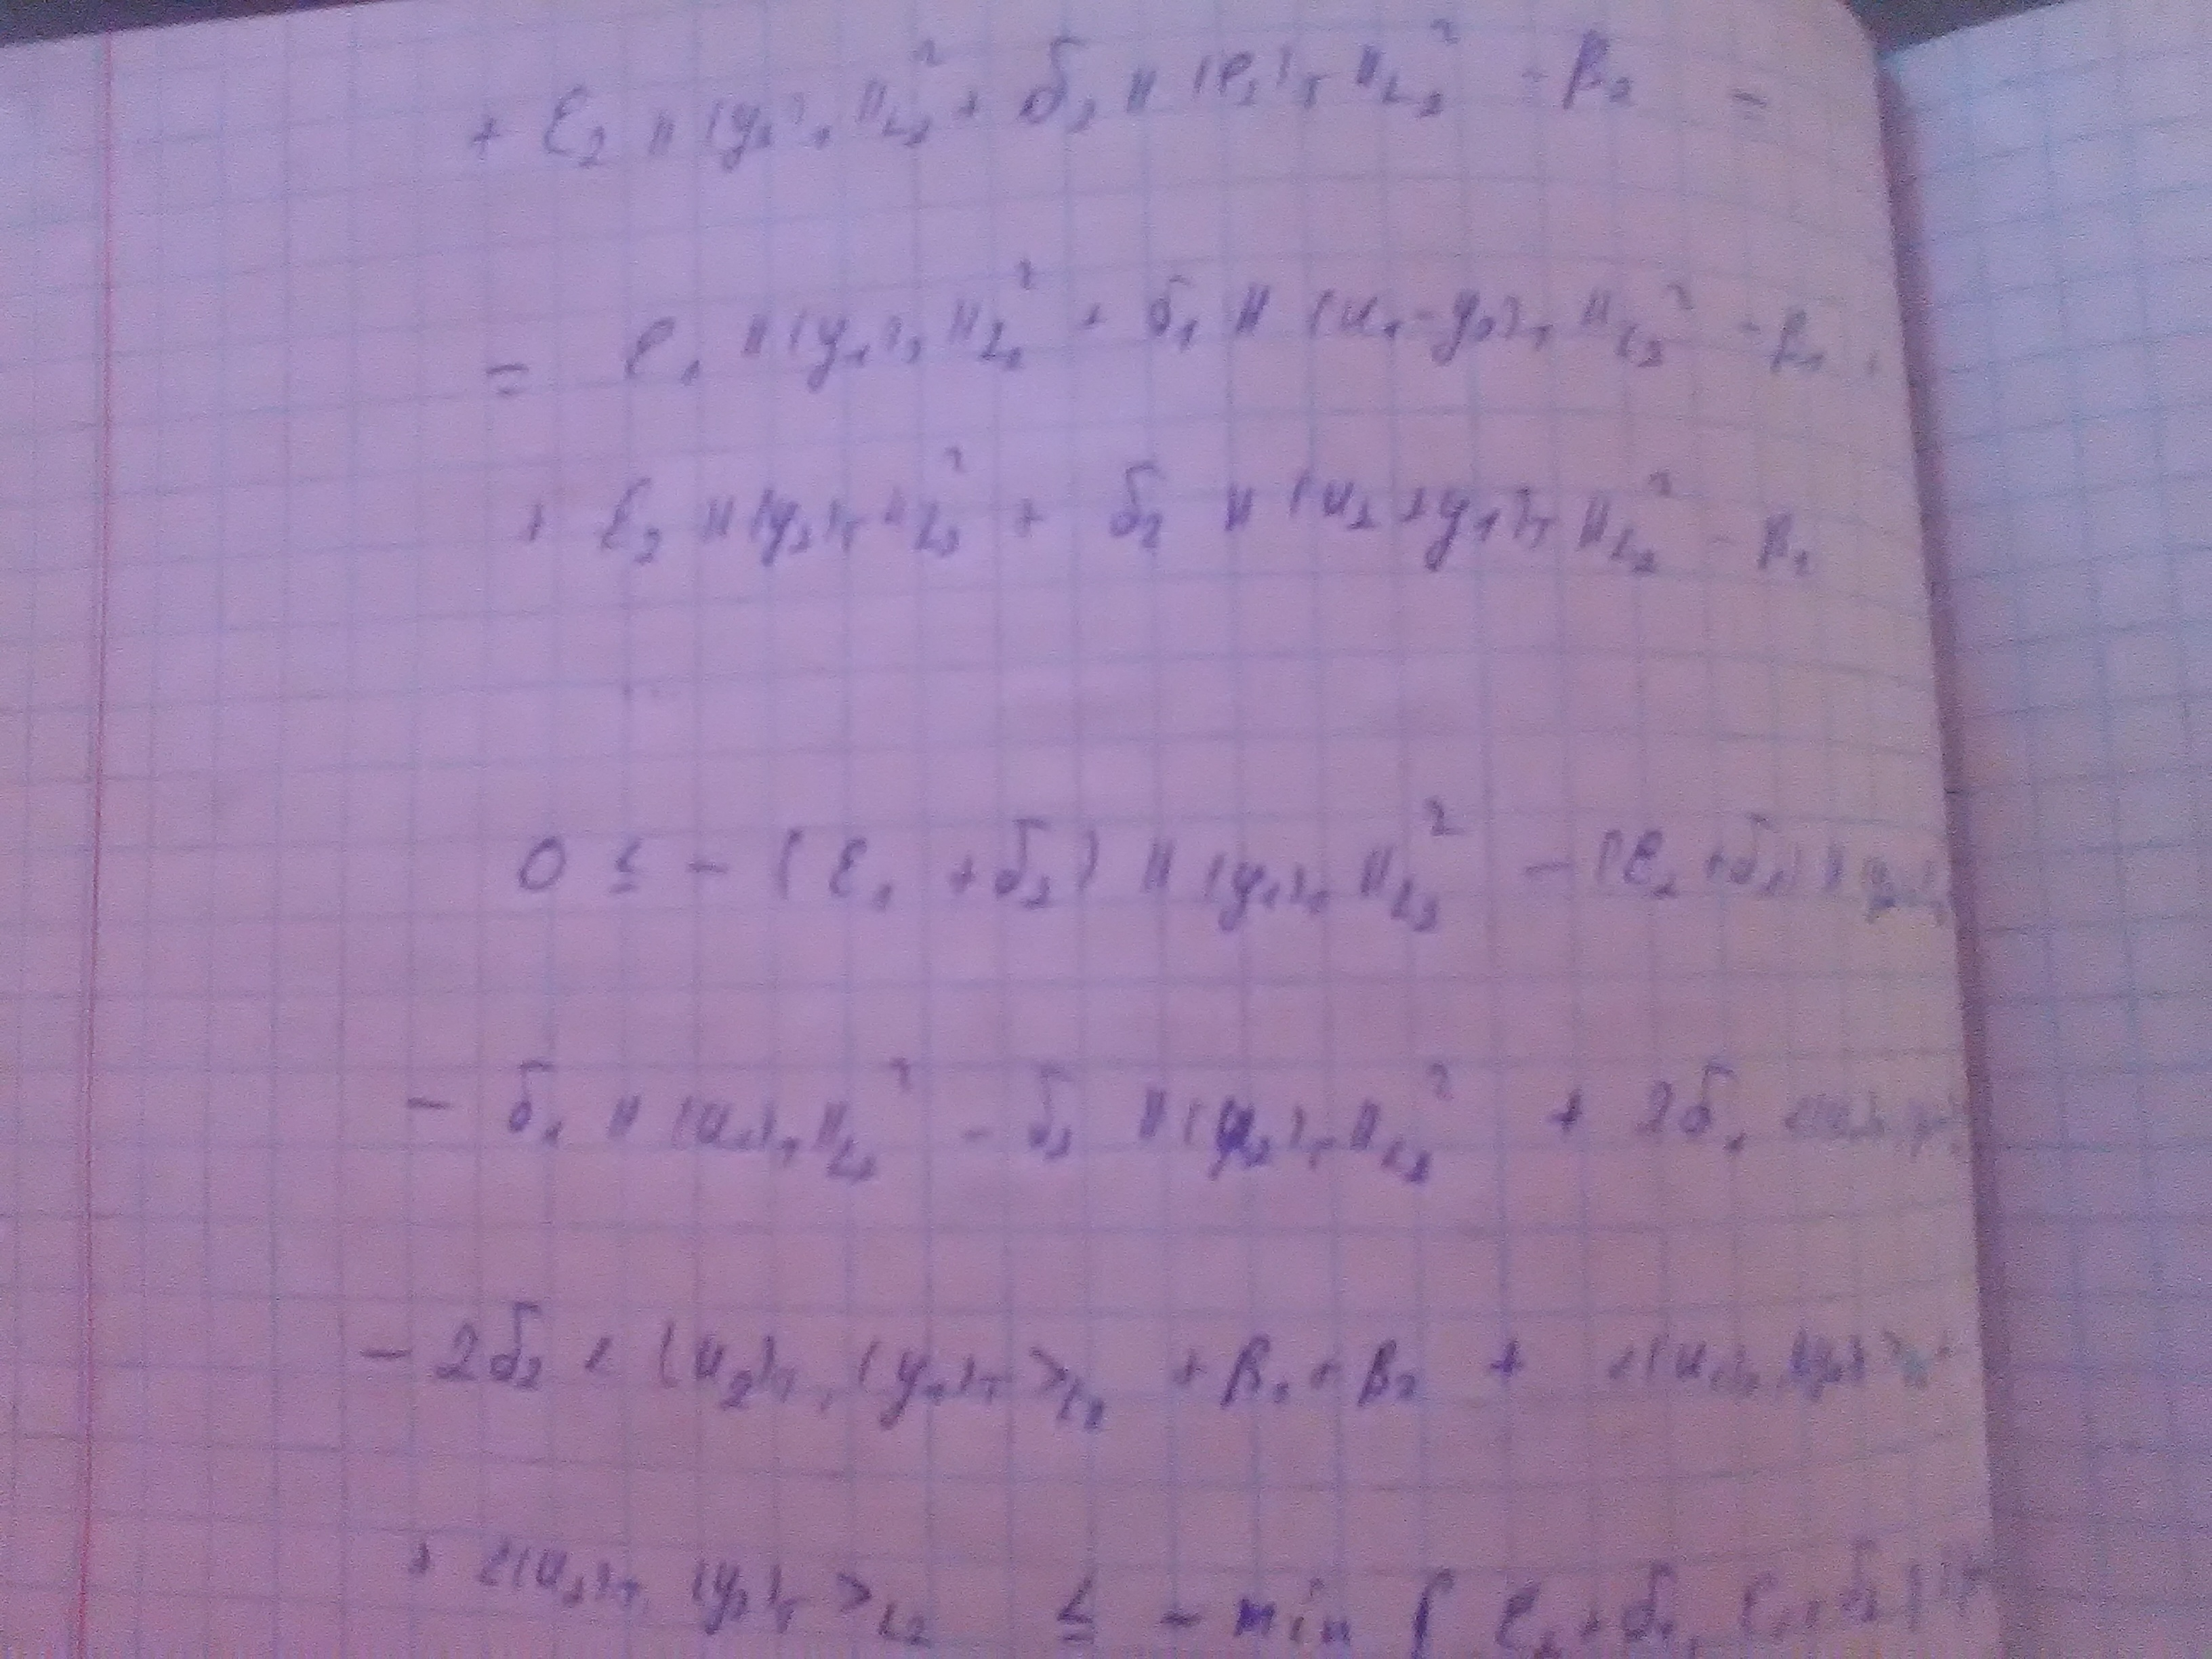
\includegraphics[scale=0.1]{10}
\end{center}
 \begin{center}
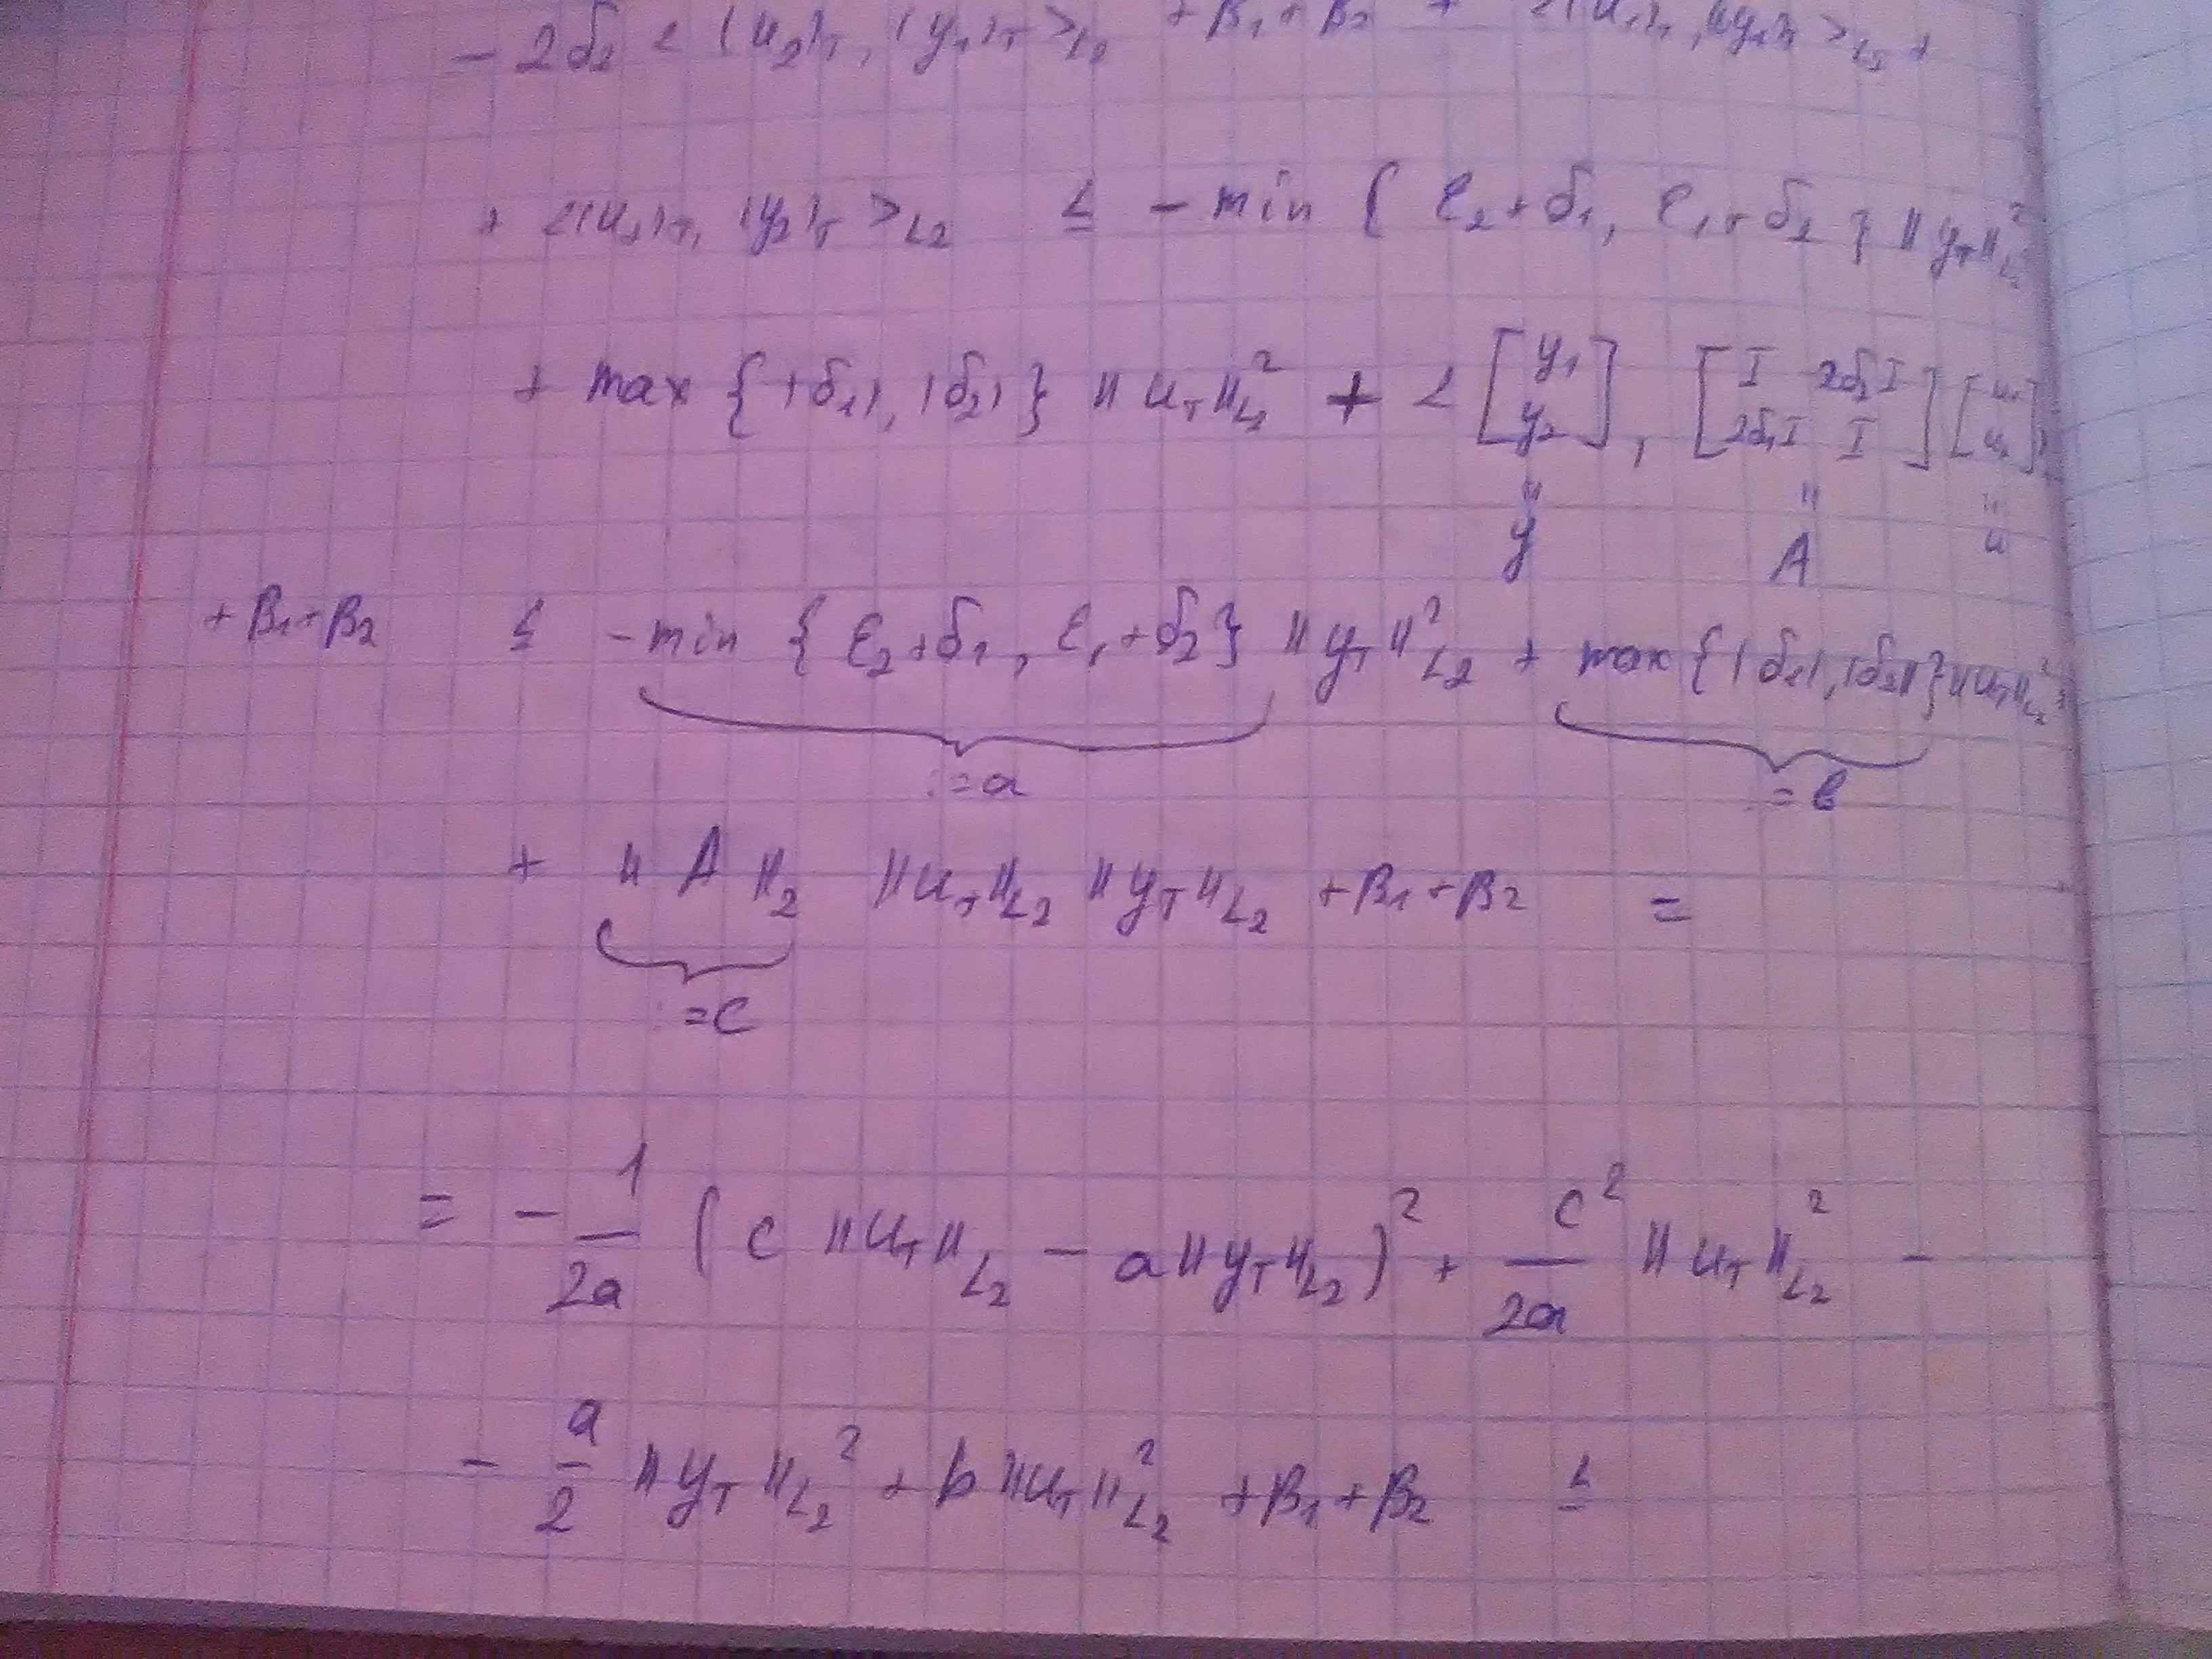
\includegraphics[scale=0.1]{11}
\end{center}
 \begin{center}
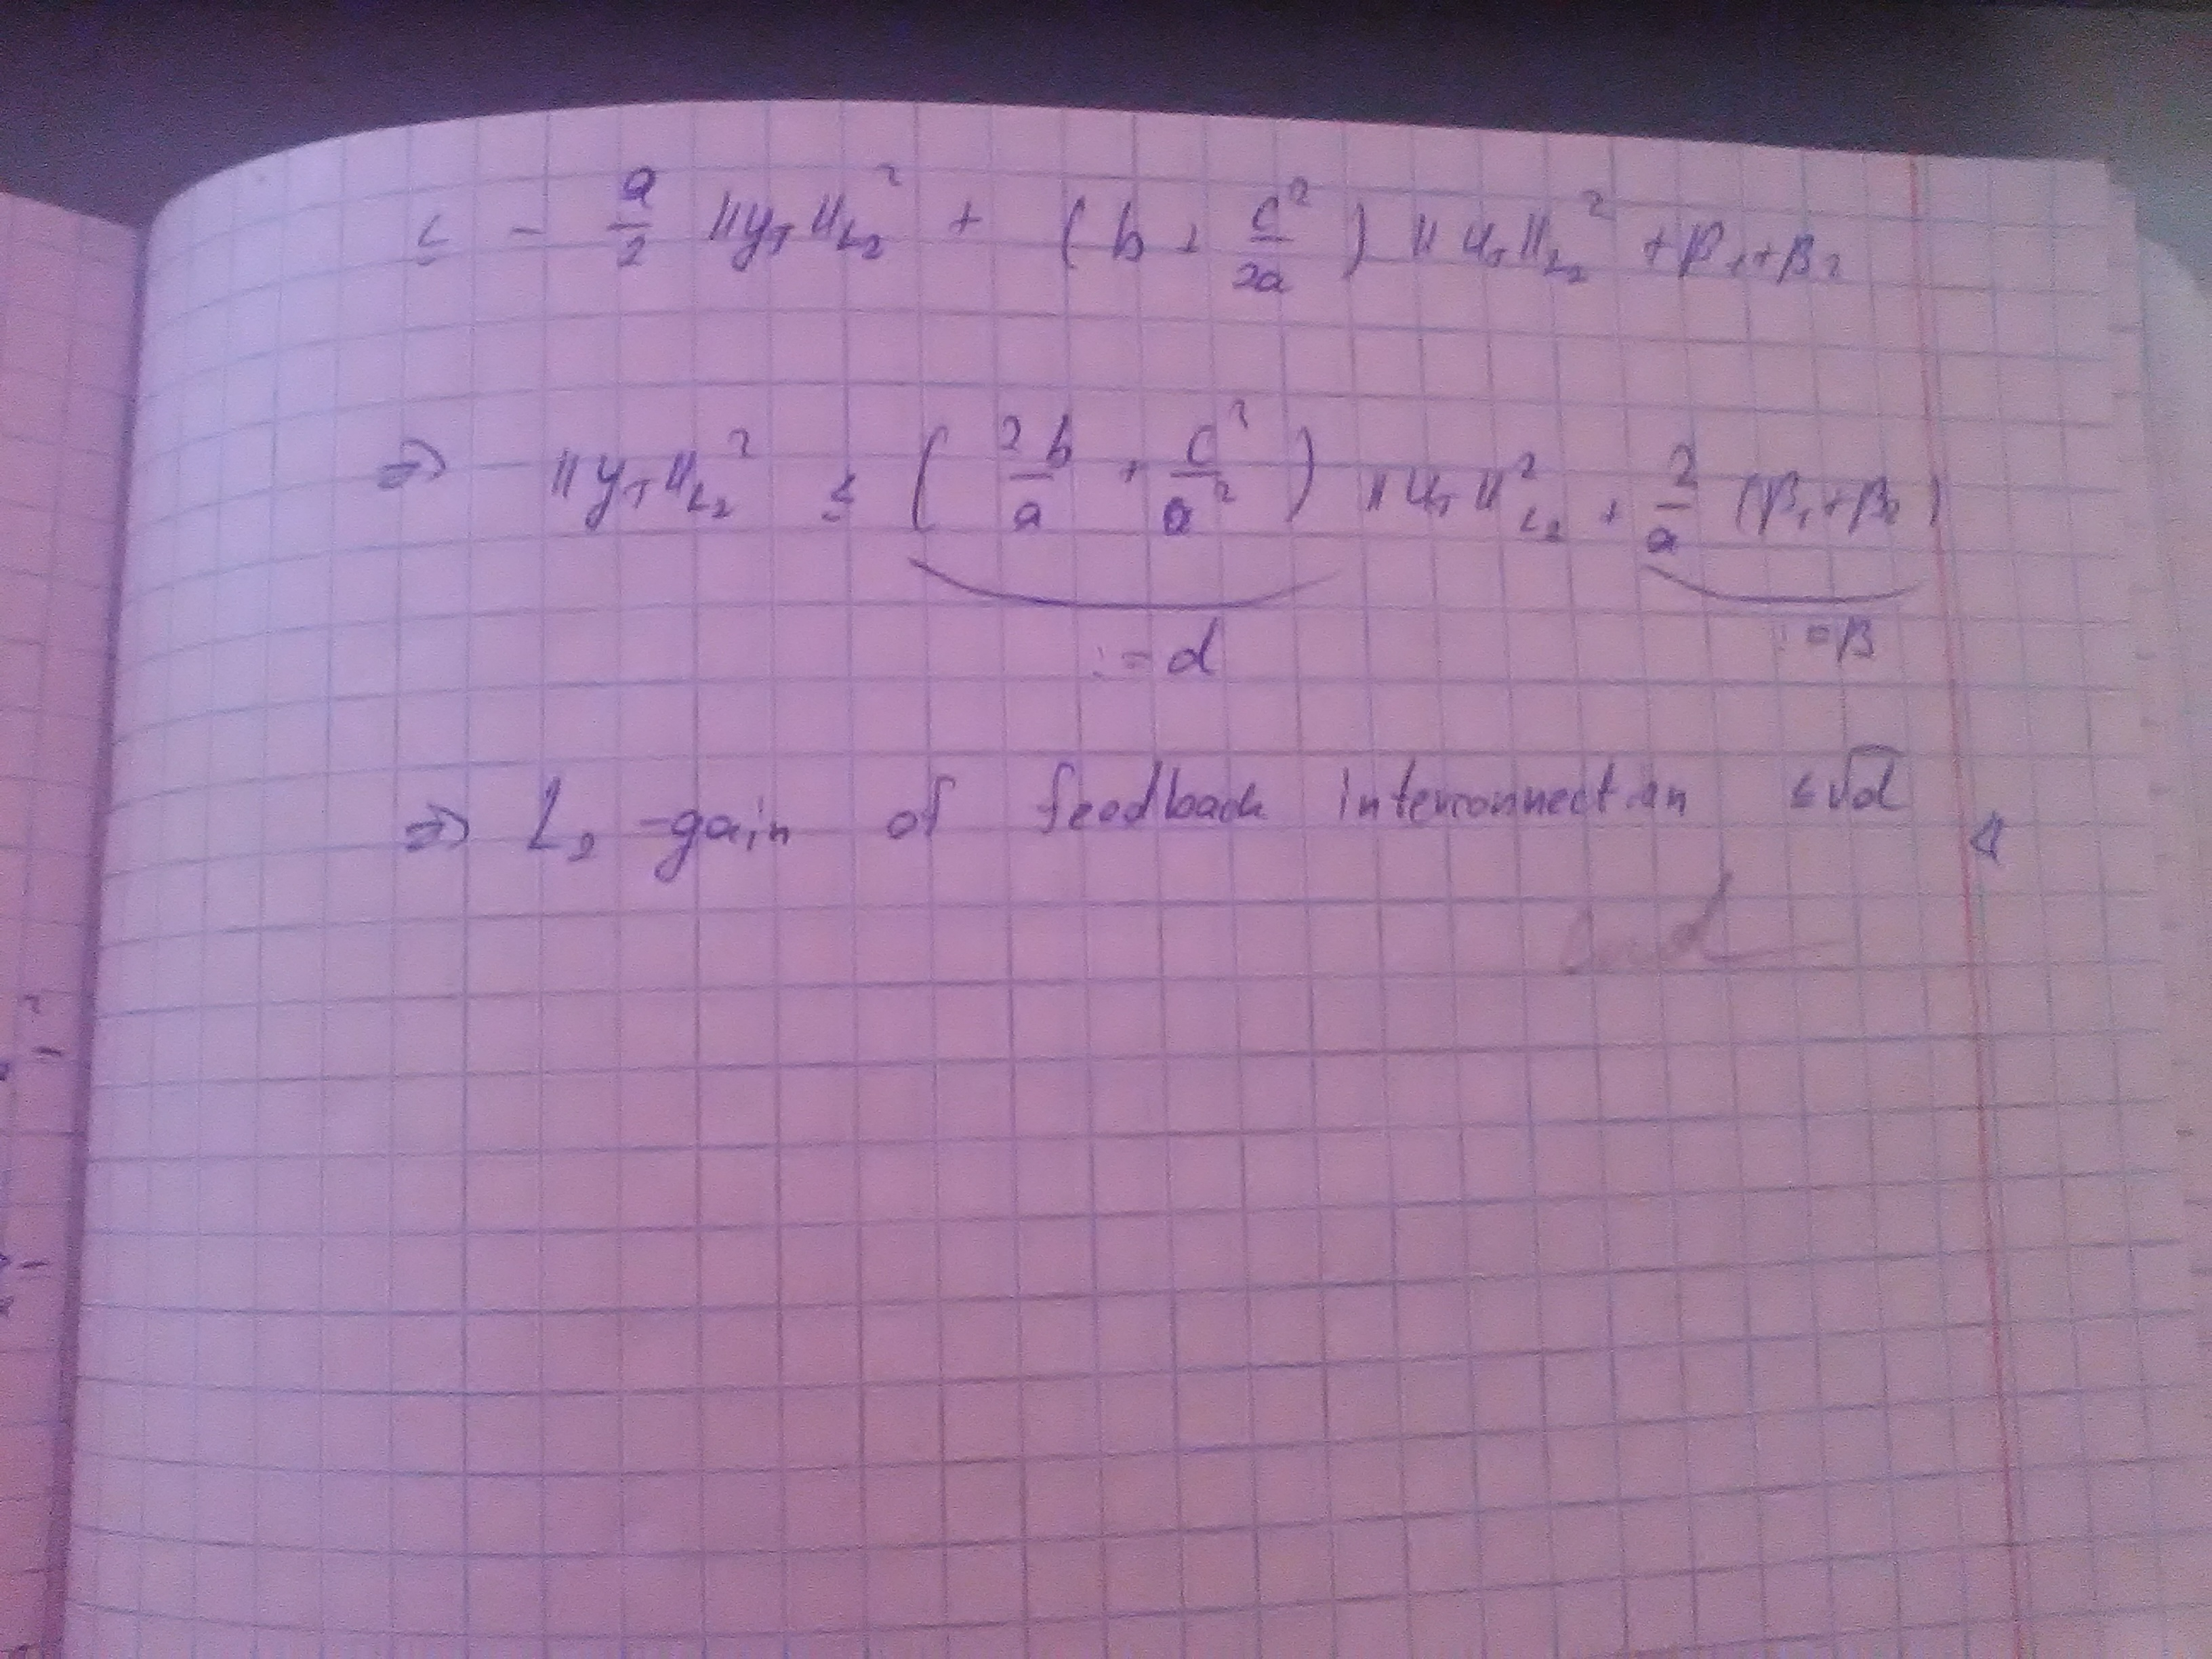
\includegraphics[scale=0.1]{12}
\end{center}
 \end{proof}
\end{Theorem}